\documentclass[10pt,spanish,aspectratio=1610]{beamer}
\usepackage[utf8]{inputenc}
\usepackage{amsmath}
\usepackage{graphicx}
\usepackage{amssymb}
\usepackage[spanish]{babel}
\spanishdecimal{.}
\usepackage{subfig}
\usepackage{fancyhdr}
\usepackage{pstricks}
\usepackage{color}
\usepackage[ruled]{algorithm2e}
\usepackage{listings}
\usepackage{multicol}
\usepackage{xcolor}

\definecolor{graywhite}{rgb}{0.9529,0.9607,0.9686}
\definecolor{bluegray}{rgb}{0.6823, 0.7411, 0.8}
\definecolor{darkred}{rgb}{0.7372, 0.2392, 0.2392}
\definecolor{bluedark}{rgb}{0.294, 0.4705, 0.6407}
\definecolor{darkgreen}{rgb}{0.1764, 0.5294, 0.0901}
\lstset{
  backgroundcolor=\color{graywhite},   % choose the background color; you must add \usepackage{color} or \usepackage{xcolor}; should come as last argument
  basicstyle=\footnotesize,        % the size of the fonts that are used for the code
  breakatwhitespace=false,         % sets if automatic breaks should only happen at whitespace
  breaklines=true,                 % sets automatic line breaking
  captionpos=b,                    % sets the caption-position to bottom
  commentstyle=\color{darkgreen},    % comment style
  keepspaces=true,                 % keeps spaces in text, useful for keeping indentation of code (possibly needs columns=flexible)
  keywordstyle=\color{darkred},       % keyword style
  language=Octave,                 % the language of the code
  morekeywords={*,...},            % if you want to add more keywords to the set
  numbers=left,                    % where to put the line-numbers; possible values are (none, left, right)
  numbersep=7pt,                   % how far the line-numbers are from the code
  numberstyle=\tiny\color{bluedark}, % the style that is used for the line-numbers
  showspaces=false,                % show spaces everywhere adding particular underscores; it overrides 'showstringspaces'
  showstringspaces=false,          % underline spaces within strings only
  showtabs=false,                  % show tabs within strings adding particular underscores
  stepnumber=1,                    % the step between two line-numbers. If it's 1, each line will be numbered
  stringstyle=\color{bluedark},     % string literal style
  frame=single,
  rulecolor=\color{bluegray},
  tabsize=2,                   % sets default tabsize to 2 spaces
  xleftmargin=1cm,
  xrightmargin=0.5cm,
  framexleftmargin=0.5cm,
  extendedchars=true,
  literate={á}{{\'a}}1 {é}{{\'e}}1 {í}{{\'i}}1 {ó}{{\'o}}1 {ú}{{\'u}}1 {Á}{{\'A}}1 {É}{{\'E}}1 {Í}{{\'I}}1 {Ó}{{\'O}}1 {Ú}{{\'U}}1,
}

\DeclareMathOperator{\atantwo}{atan2}
\setbeamercolor{block title}{fg=white,bg=blue!70!black}
\setbeamercolor{block body}{fg=black, bg=blue!10!white}
\setbeamertemplate{blocks}[rounded][shadow=false]
\setbeamercovered{transparent}
\beamertemplatenavigationsymbolsempty
\setbeamertemplate{frametitle}{
  \leavevmode
  \hbox{\begin{beamercolorbox}[wd=0.6\paperwidth,left]{frametitle}
    \usebeamerfont{frametitle}\insertframetitle
  \end{beamercolorbox}
  \begin{beamercolorbox}[wd=0.4\paperwidth,center]{frametitle}
    \usebeamerfont{frametitle}\small{\thesection . \insertsectionhead}
  \end{beamercolorbox}  } }
\setbeamertemplate{footline}{
  \leavevmode%
  \hbox{%
    \begin{beamercolorbox}[colsep=-0.5pt,wd=.33\paperwidth,ht=3ex,dp=1.5ex,center]{author in head/foot}%
      \usebeamerfont{author in head/foot}\insertshortauthor~~ (\insertshortinstitute)
    \end{beamercolorbox}%
    \begin{beamercolorbox}[colsep=-0.5pt,wd=.34\paperwidth,ht=3ex,dp=1.5ex,center]{date in head/foot}%
      \usebeamerfont{author in head/foot}\insertshorttitle
    \end{beamercolorbox}%
    \begin{beamercolorbox}[colsep=-0.5pt,wd=.33\paperwidth,ht=3ex,dp=1.5ex,right]{author in head/foot}%
      \usebeamerfont{author in head/foot}\insertshortdate{} \hspace*{2em}\scriptsize{\insertframenumber{}}\hspace*{1ex}
    \end{beamercolorbox}
  }
}

\begin{document}
\renewcommand{\tablename}{Tabla}
\renewcommand{\figurename}{Figura}

\title[Tareas Básicas en Robots de Servicio Doméstico]{Tareas Básicas en Robots de Servicio Doméstico}
\author[Marco Negrete]{Instructor: Dr. Marco Antonio Negrete Villanueva}
\institute[FI, UNAM]{Facultad de Ingeniería, UNAM}
\date[EIR 2023]{Escuela de Invierno de Robótica 2023\\Zacatecas\\\url{https://github.com/mnegretev/EIR-2023-AtHomeBasicTasks}}

\begin{frame}
\titlepage
\end{frame}

\begin{frame}
  \Large{Objetivos:}
  \normalsize
  \[\]
  \textbf{Objetivo General:} Brindar los conocimientos básicos necesarios para desarrollar un robot de servicio doméstico.
  \\
  \textbf{Objetivos Específicos:}
  \begin{itemize}
  \item Revisar el hardware necesario para tener un robot de servicio doméstico: sensores y actuadores más comunes.
  \item Dar un panorama general del software necesario para desarrollar un robot de servicio doméstico.
  \item Revisar las herramientas disponibles para cubrir las habilidades básicas requeridas en un robot de servicio doméstico:
    \begin{itemize}
    \item Navegación
    \item Vision
    \item Manipulación
    \item Síntesis y reconocimiento de voz
    \item Planeación de acciones
    \end{itemize}
  \end{itemize}
\end{frame}

\begin{frame}
  \Large{Contenido}
  \normalsize
  \[\]

  \tableofcontents
\end{frame}


\section{Introducción}

\begin{frame}
  \Huge
  Introducción
\end{frame}

\begin{frame}\frametitle{Los robots de servicio doméstico}
  \begin{columns}
    \begin{column}{0.5\textwidth}
      Son robots pensados para ayudar en tareas comunes del hogar u oficina. Requieren de varias habilidades:
      \begin{itemize}
      \item Interacción humano-robot
      \item Navegación en ambientes dinámicos
      \item Reconocimiento de objetos
      \item Manipulación de objetos
      \item Comportamientos adaptables
      \item Planeación de acciones
      \end{itemize}
    \end{column}
    \begin{column}{0.4\textwidth}
      \centering
      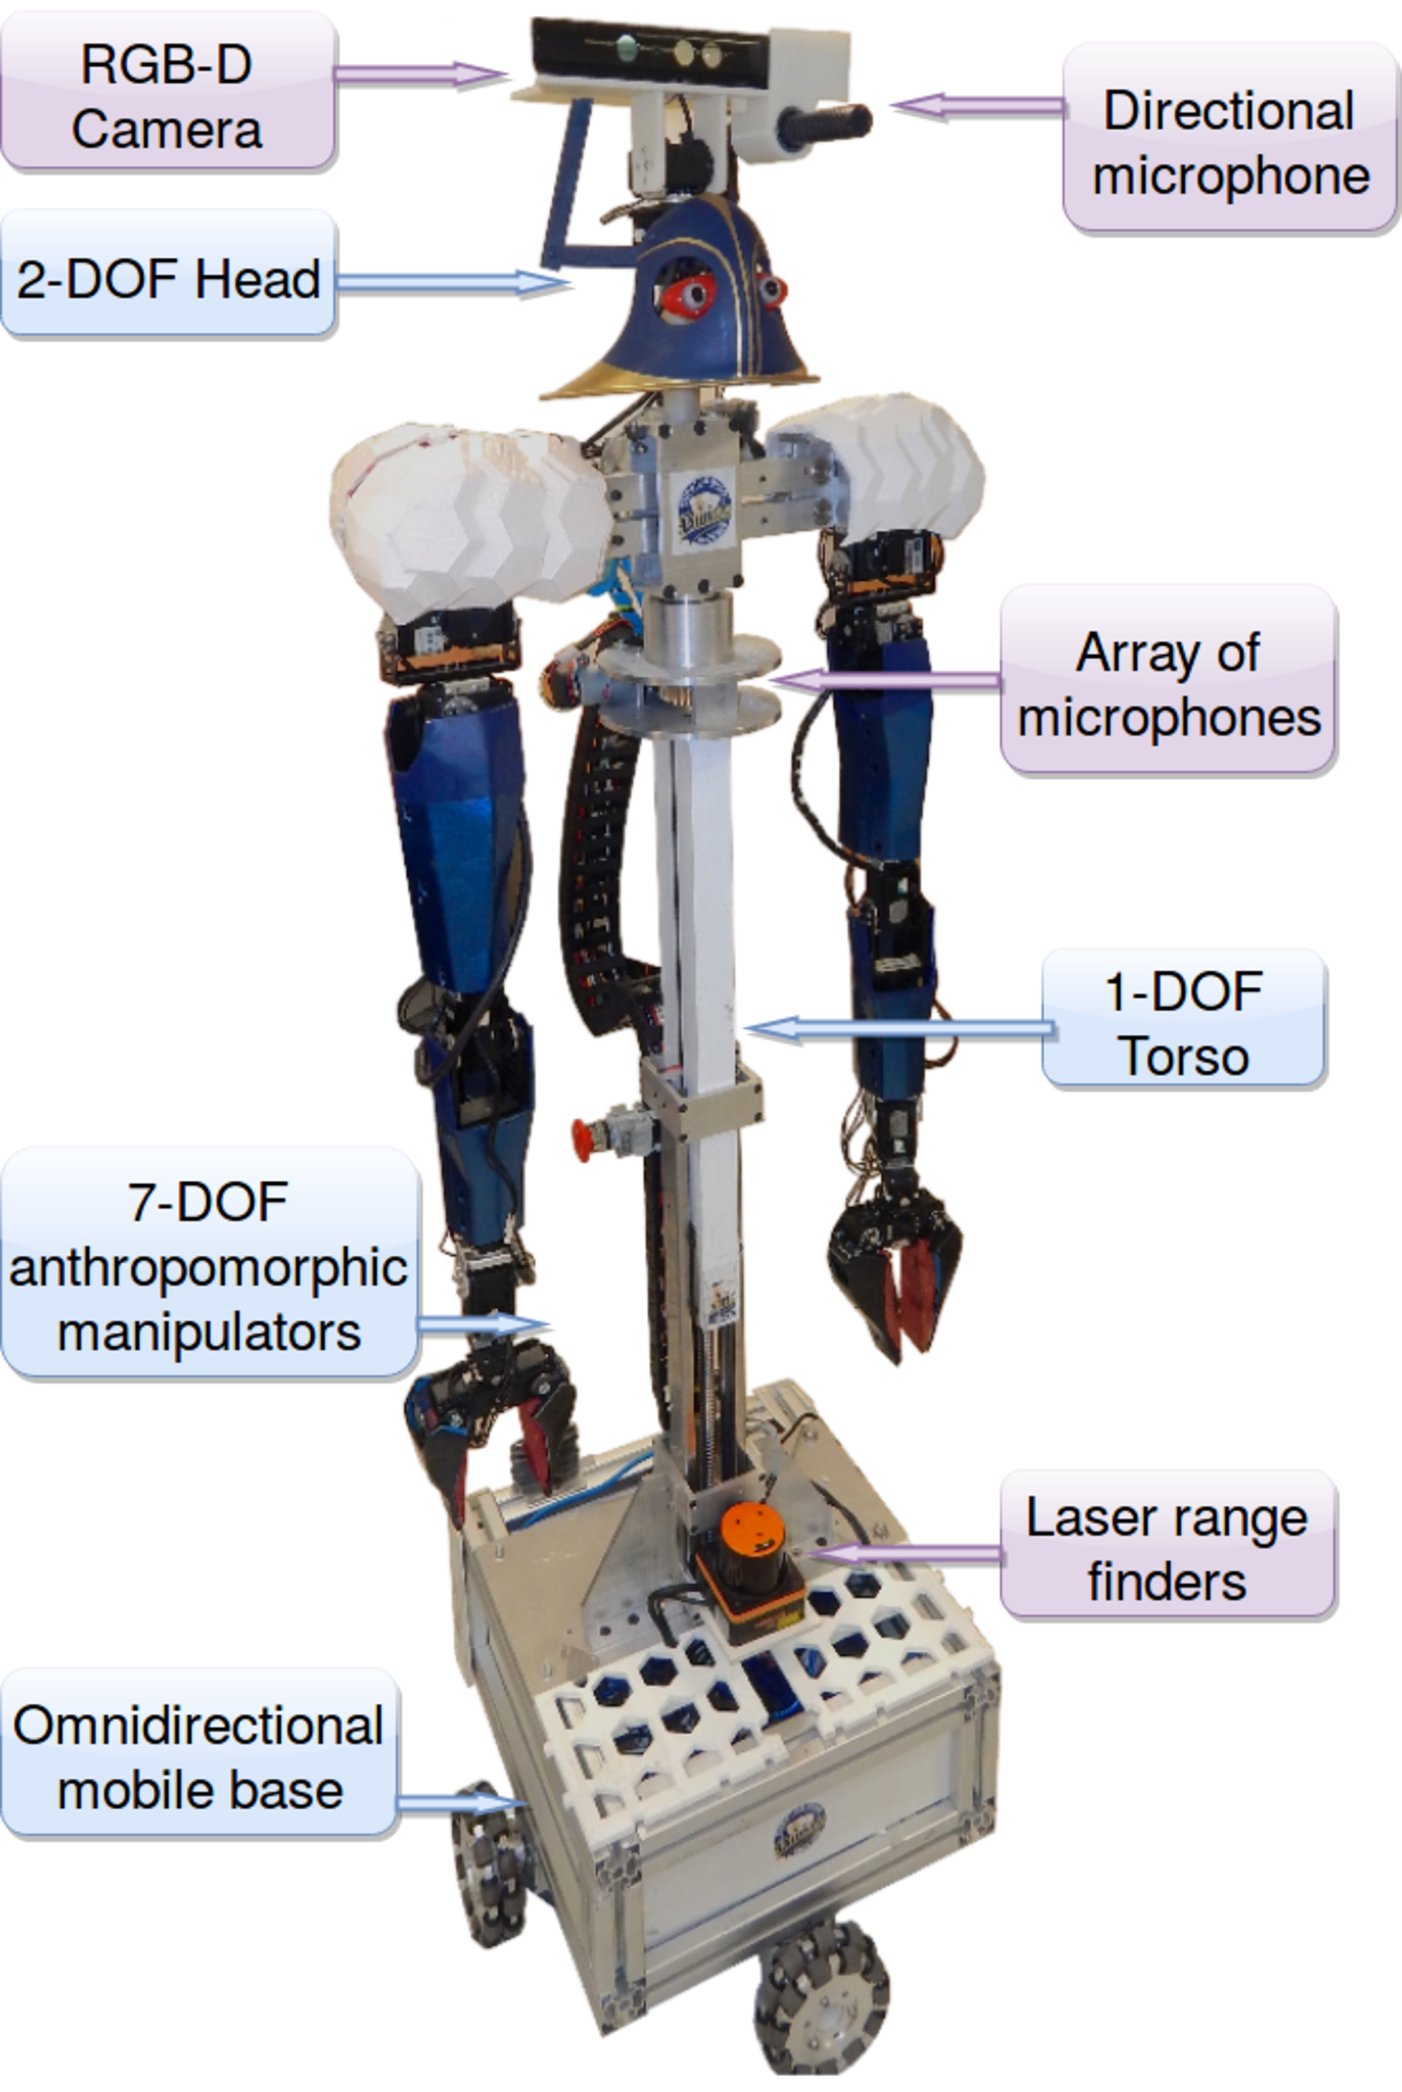
\includegraphics[width=0.9\textwidth]{Figures/Justina.pdf}
    \end{column}
  \end{columns}
\end{frame}

\begin{frame}\frametitle{Hardware necesario: Base móvil}
  \begin{columns}
    \begin{column}{0.5\textwidth}
      \begin{itemize}
      \item De preferencia, debe ser omnidireccional
      \item Turtle Bot (\url{https://www.turtlebot.com/})
      \item Festo Robotino (\url{https://wiki.openrobotino.org/})
      \item DIY: 3 ó 4 motores de corriente directa con ruedas omnidireccionales, 2 tarjetas Roboclaw, baterías de LiPo y chasis de alumnio estructural.
      \end{itemize}
    \end{column}
    \begin{column}{0.5\textwidth}
      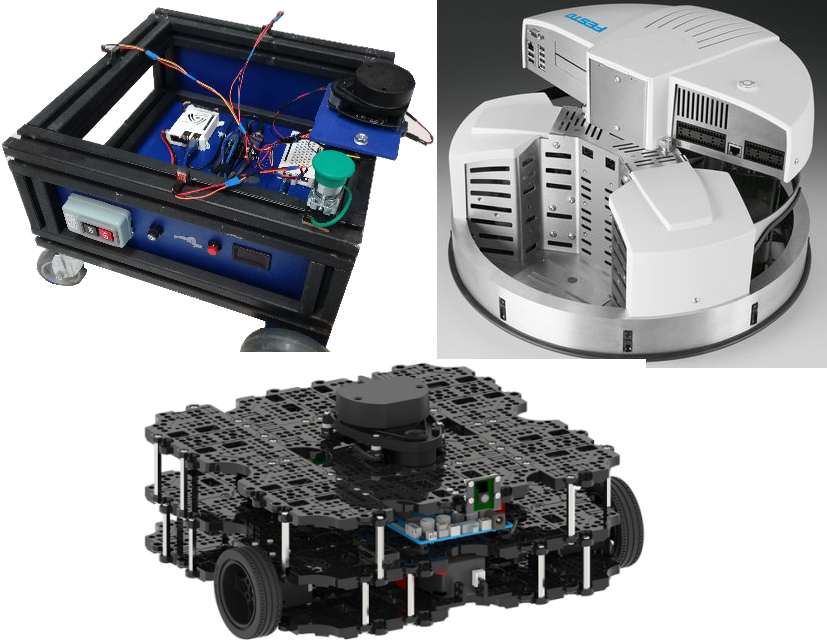
\includegraphics[width=\textwidth]{Figures/Bases.png}
    \end{column}
  \end{columns}
\end{frame}

\begin{frame}\frametitle{Hardware necesario: Cámaras}
  \begin{columns}
    \begin{column}{0.45\textwidth}
      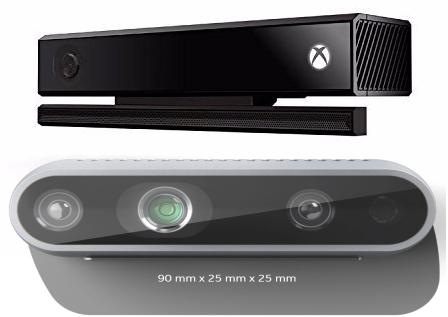
\includegraphics[width=\textwidth]{Figures/Cameras.jpg}
    \end{column}
    \begin{column}{0.5\textwidth}
      \begin{itemize}
      \item Se pueden usar sólo cámaras RGB, pero es altamente recomendable tener información de profundidad.
      \item Kinect (\url{https://github.com/OpenKinect/libfreenect2})
      \item Intel RealSense (\url{https://github.com/IntelRealSense/librealsense})
      \item También se pueden usar cámaras estéreo, pero es mucho más sencillo usar cámaras con luz estructurada.
      \end{itemize}
    \end{column}
  \end{columns}
\end{frame}

\begin{frame}\frametitle{Hardware necesario: Sensor láser}
  \begin{columns}
    \begin{column}{0.5\textwidth}
      \begin{itemize}
      \item Hokuyo (\url{https://www.hokuyo-aut.jp/})
      \item RPLidar (\url{https://www.robotshop.com/en/slamtec.html})
      \item SICK (\url{https://www.sick.com/ag/en/detection-and-ranging-solutions/2d-lidar-sensors/c/g91900})
      \item El paquete \url{http://wiki.ros.org/urg_node} facilita su operación.
      \item Si no se tiene uno, se puede simular a partir de una cámara RGB-D con el paquete \url{http://wiki.ros.org/pointcloud_to_laserscan}.
      \end{itemize}
    \end{column}
    \begin{column}{0.4\textwidth}
      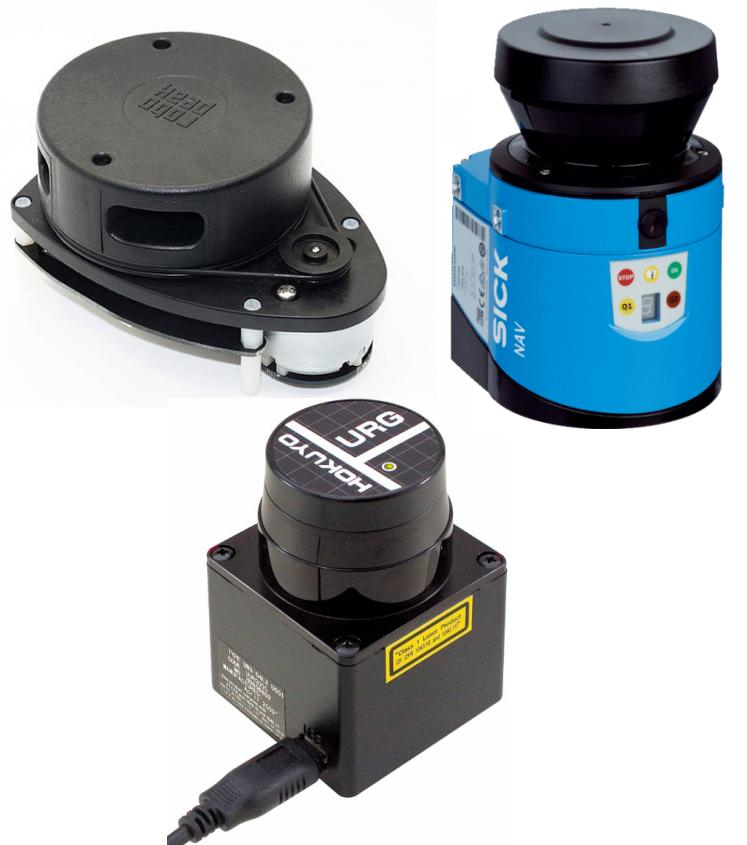
\includegraphics[width=\textwidth]{Figures/lasers.jpg}
    \end{column}
  \end{columns}
\end{frame}

\begin{frame}\frametitle{Hardware necesario: Manipulador}
  \begin{columns}
    \begin{column}{0.4\textwidth}
      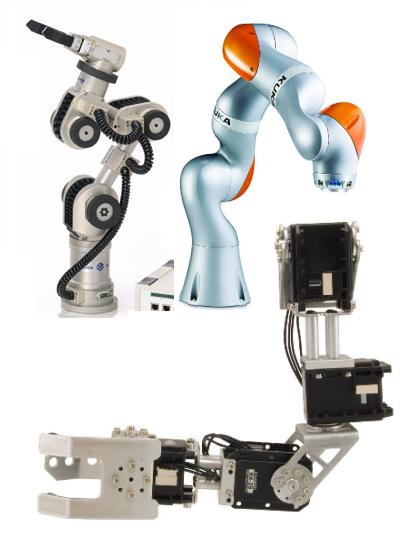
\includegraphics[width=\textwidth]{Figures/arms.jpg}
    \end{column}
    \begin{column}{0.5\textwidth}
      \begin{itemize}
      \item Son recomendables por lo menos 5 DOF.
      \item Kuka LBR iiwa (\url{http://wiki.ros.org/kuka})
      \item Neuronics Katana (\url{http://wiki.ros.org/katana})
      \item DIY: Servomotores y Brackets Dynamixel (\url{http://wiki.ros.org/dynamixel})
      \end{itemize}
    \end{column}
  \end{columns}
\end{frame}

\section{ROS}

\begin{frame}
  \Huge
  La plataforma ROS
\end{frame}


\begin{frame}\frametitle{La plataforma ROS}
  
\includegraphics[width=0.3\textwidth]{Figures/Ros_logo.png}
  \[\]
  \textbf{ROS (Robot Operating System) } es un \textit{middleware} de código abierto para el desarrollo de robots móviles.
  \begin{itemize}
  \item Implementa funcionalidades comúnmente usadas en el desarrollo de robots como el paso de mensajes entre procesos y la administración de paquetes.
  \item Muchos drivers y algoritmos ya están implementados.
  \item Es una plataforma distribuida de procesos (llamados \textit{nodos}).
  \item Facilita el reuso de código.
  \item Independiente del lenguaje (Python y C++ son los más usados).
  \item Facilita el escalamiento para proyectos de gran escala. 
  \end{itemize}
\end{frame}

\begin{frame}\frametitle{Conceptos}
  ROS se puede entender en dos grandes niveles conceptuales:
  \begin{itemize}
  \item \textbf{Sistema de archivos:} Recursos de ROS en disco
  \item \textbf{Grafo de procesos:} Una red \textit{peer-to-peer} de procesos (llamados nodos) en tiempo de ejecución.
  \end{itemize}
\end{frame}

\begin{frame}\frametitle{Sistema de archivos}
  \begin{columns}
    \begin{column}{0.5\textwidth}
      Recursos en disco:
      \begin{itemize}
      \item \textbf{Workspace:} carpeta que contiene los paquete desarrollados
      \item \textbf{Paquetes:} Principal unidad de organización del software en ROS (concepto heredado de Linux)
      \item \textbf{Manifiesto:} (\texttt{package.xml}) provee metadatos sobre el paquete (dependencias, banderas de compilación, información del desarrollador)
      \item \textbf{Mensajes (msg):} Archivos que definen la estructura de un \textit{mensaje} en ROS.
        \item \textbf{Servicios (srv):} Archivos que definen las estructuras de la petición (\textit{request}) y respuesta (\textit{response}) de un servicio. 
      \end{itemize}
    \end{column}
    \begin{column}{0.4\textwidth}
      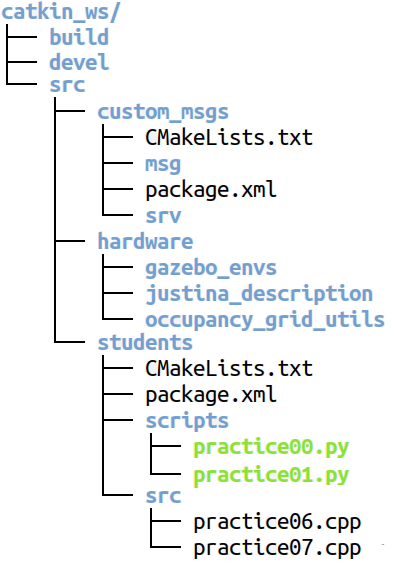
\includegraphics[width=\textwidth]{Figures/catkin_tree.png}
    \end{column}
  \end{columns}
\end{frame}

\begin{frame}\frametitle{Grafo de procesos}
  El grafo de procesos es una red \textit{peer-to-peer} de programas (nodos) que intercambian información entre sí. Los principales componentes del este grafo son:
  \[\]
  \begin{columns}
    \begin{column}{0.5\textwidth}
      \begin{itemize}
      \item master
      \item servidor de parámetros
      \item nodos
      \item mensajes
      \item servicios 
      \end{itemize}
    \end{column}
    \begin{column}{0.5\textwidth}
      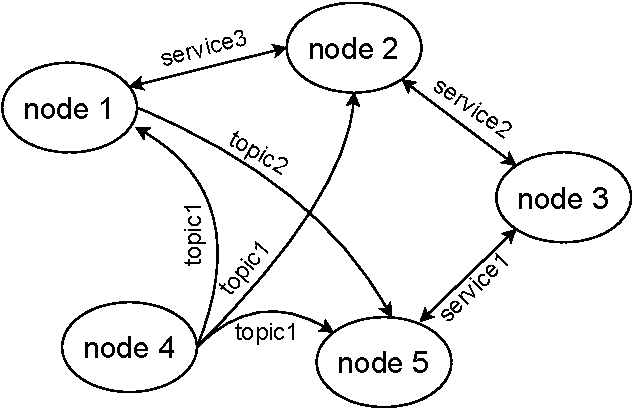
\includegraphics[width=\textwidth]{Figures/RosGraph.pdf}
    \end{column}
  \end{columns}
\end{frame}

\begin{frame}\frametitle{Tópicos y servicios}
  Los nodos (procesos) en ROS intercambian información a través de dos grandes patrones:
  \[\]
  \begin{columns}
    \begin{column}{0.6\textwidth}
        \begin{itemize}
        \item \textbf{Tópicos}
          \begin{itemize}
          \item Son un patrón $1:n$ de tipo \textit{publicador/suscriptor}
          \item Son no bloqueantes
          \item Utilizan estructuras de datos definidas en archivos \texttt{*.msg} para el envío de información
          \end{itemize}
        \item \textbf{Servicios}
          \begin{itemize}
          \item Son un patrón $1:1$ de tipo \textit{petición/respuesta}
          \item Son bloqueantes
          \item Utilizan estructuras de datos definidas en archivos \texttt{*.srv} para el intercambio de información. 
          \end{itemize}
        \end{itemize}
    \end{column}
    \begin{column}{0.4\textwidth}
      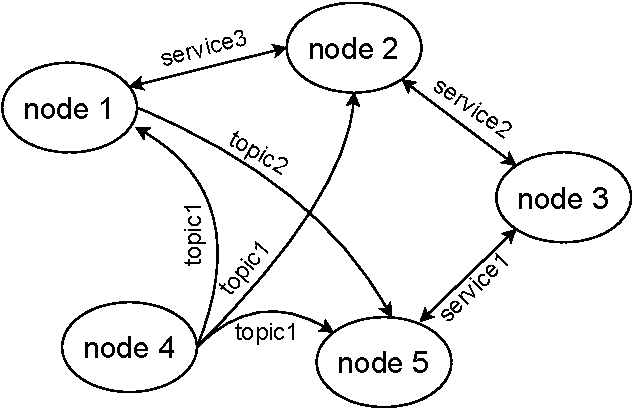
\includegraphics[width=\textwidth]{Figures/RosGraph.pdf}
    \end{column}
  \end{columns}
  \[\]
  Para mayor información:
  \begin{itemize}
  \item Tutoriales \url{http://wiki.ros.org/ROS/Tutorials}
  \item Koubâa, A. (Ed.). (2020). Robot Operating System (ROS): The Complete Reference. Springer Nature
  \end{itemize}
\end{frame}

%\section{Conceptos Básicos}

\begin{frame}
  \Huge
  Conceptos básicos
\end{frame}

\begin{frame}\frametitle{Funciones comunes}
  \textbf{Sigmoide}: Es una función que puede ser usada como una versión \textit{suave} del escalón. Se usará en en control de posición y en el entrenamiento de redes neuronales.
  \[\sigma(x) = \frac{1}{1 + e^{-x}}\]
  La derivada tiene la forma:
  \[\frac{d\sigma}{dx}=\frac{-(-e^{-x})}{\left(1 + e^{-x}\right)^2} = \frac{1 + e^{-x} - 1}{\left(1 + e^{-x}\right)^2}=\frac{1}{1+e^{-x}}\left(1 - \frac{1}{1 + e^{-x}}\right) = \sigma(x)(1 - \sigma(x))\]
  \textbf{Campana de Gauss}: Es una función siempre positiva que tiende a cero cuando $|x|\rightarrow \infty$:
  \[f(x) = a \cdot e^{-\frac{(x - b)^2}{2c^2}}\]
\end{frame}

\begin{frame}\frametitle{Gradiente}
  Dada una función $f:\mathbb{R}^n \rightarrow \mathbb{R}$, es decir, una función escalar de variable vectorial $f(x_1, x_2, \dots, x_n)$, el gradiente $\nabla f(\bar{x})$ está dado por:
  \[\nabla f(\bar{x}) = \left[ \frac{\partial f}{\partial x_1}, \frac{\partial f}{\partial x_2}, \dots \frac{\partial f}{\partial x_n}\right]^T\]

  \begin{itemize}
  \item El gradiente generaliza el concepto de derivada para funciones de varias variables.
  \item El gradiente evaluado en un punto $\bar{x}_0$ indica la dirección de máximo cambio en ese punto.
  \end{itemize}
\end{frame}

\begin{frame}\frametitle{Jacobiano}
  Dada una función $F:\mathbb{R}^n \rightarrow \mathbb{R}^m$, es decir, una función vectorial de variable vectorial:
  \[F(\bar{x}) = \begin{tabular}{l}$f_1(x_1, x_2, ..., x_n)$\\$f_2(x_1, x_2, ..., x_n)$\\ $\vdots$ \\ $f_n(x_1, x_2, ..., x_n)$\end{tabular}\]
  El Jacobiano es una matriz que contiene las primeras derivadas parciales:
  \[J(x) = \left[\begin{tabular}{cccc}
      $\dfrac{\partial f_1}{\partial x_1}$ & $\dfrac{\partial f_1}{\partial x_2}$ & $\dots$ & $\dfrac{\partial f_1}{\partial x_n}$\\
      & & &\\
      $\dfrac{\partial f_2}{\partial x_1}$ & $\dfrac{\partial f_2}{\partial x_2}$ & $\dots$ & $\dfrac{\partial f_2}{\partial x_n}$\\
      & $\vdots$ & & \\
      $\dfrac{\partial f_m}{\partial x_1}$ & $\dfrac{\partial f_m}{\partial x_2}$ & $\dots$ & $\dfrac{\partial f_m}{\partial x_n}$\\
    \end{tabular}\right] = \left[\begin{tabular}{c}$\nabla^T f_1$\\ $\nabla^T f_2$ \\ $\vdots$ \\ $\nabla^T f_m$\end{tabular}\right]\in\mathbb{R}^{m\times n}\]
\end{frame}

\begin{frame}\frametitle{Espacio de Configuraciones}
  La \textit{configuración} de un robot (o de una parte de él) es una descripción de todos los puntos que ocupa en el espacio. Los \textit{grados de libertad} son el conjunto mínimo de valores independientes que se requieren para definir una configuración.
  \[\]
  La configuración de un cuerpo rígido que se mueve en el espacio tiene 6 grados de libertad (tres para posición y tres para orientación): $(x,y,z,\psi,\theta,\phi)$. Si el cuerpo se mueve sólo en el plano, tiene 3 grados: $(x,y,\theta)$ (una posición en 2D y una orientación).
\end{frame}


\section[Navegación]{Navegación}

\begin{frame}
  \Huge
  Navegación
\end{frame}

\begin{frame}\frametitle{Planeación de movimientos}
  El problema de la planeación de movimientos comprende cuatro tareas principales:
  \begin{itemize}
  \item Navegación: encontrar un conjunto de puntos $q \in Q_{free}$ que permitan al robot moverse desde una configuración inicial $q_{start}$ a una configuración final $q_{goal}$. 
  \item Mapeo: construir una representación del ambiente a partir de las lecuras de los sensores y la trayectoria del robot. 
  \item Localización: determinar la configuración $q$ dado un mapa y lecturas de los sensores. 
  \item Barrido: pasar un actuador por todos los puntos $q\in Q_b \subset Q$.
  \end{itemize}
\end{frame}

\begin{frame}\frametitle{Representación del ambiente}
  Un mapa es cualquier representación del ambiente útil en la toma de decisiones.
  \begin{itemize}
  \item Interiores (se suelen representar en 2D)
    \begin{itemize}
    \item Celdas de ocupación
    \item Mapas de líneas
    \item Mapas topológicos: Diagramas de Voronoi generalizados. 
    \item Mapas basados en \textit{Landmarks}
    \end{itemize}
  \item Exteriores (suelen requerir una representación 3D)
    \begin{itemize}
    \item Celdas de elevación
    \item Celdas de ocupación 3D
    \item Octomaps
    \end{itemize}
  \end{itemize}
\end{frame}

\begin{frame}\frametitle{Celdas de ocupación}
  Es un tipo de mapa geométrico. El espacio se discretiza con una resolución determinada y a cada celda se le asigna un número $p\in[0,1]$ que indica su nivel de ocupación. En un enfoque probabilístico este número se puede interpretar como la certeza que se tiene de que una celda esté ocupada.
  \begin{figure}
    \centering
    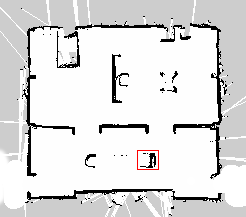
\includegraphics[width=0.4\textwidth]{Figures/OccupancyGrid.png}
    
\includegraphics[width=0.4\textwidth]{Figures/UniversumZoom.png}
    \end{figure}
  El mapa resultante se representa en memoria mediante una matriz de valores de ocupación. En ROS, los mapas utilizan el mensaje \texttt{nav\_msgs/OccupancyGrid}.
\end{frame}

\begin{frame}[containsverbatim]\frametitle{Ejercicio 1 - Celdas de ocupación}
  \begin{enumerate}
  \item Abra una terminal (Ctrl + Alt + t) y ejecute el comando \texttt{roslaunch bring\_up path\_planning.launch}
  \item Inspeccione el mapa de celdas de ocupación
  \item Detenga la ejecución (Ctrl + C)
  \item Abra el archivo \texttt{catkin\_ws/src/config\_files/maps/appartment.pgm} con cualquier editor de imágenes y realice alguna modificación (puede ser agregar una mancha negra o borrar algún obstáculo).
  \item Ejecute de nuevo la simulación y observe los cambios
  \end{enumerate}
\end{frame}

\begin{frame}\frametitle{Inflado de celdas de ocupación}
  Aunque las celdas de ocupación representan el espacio donde hay obstáculos y donde no, en realidad, el robot no puede posicionarse en todas las celdas libres, debido a su tamaño, como se observa en la figura:
  \begin{columns}
    \begin{column}{0.6\textwidth}
      \begin{figure}
        \centering
        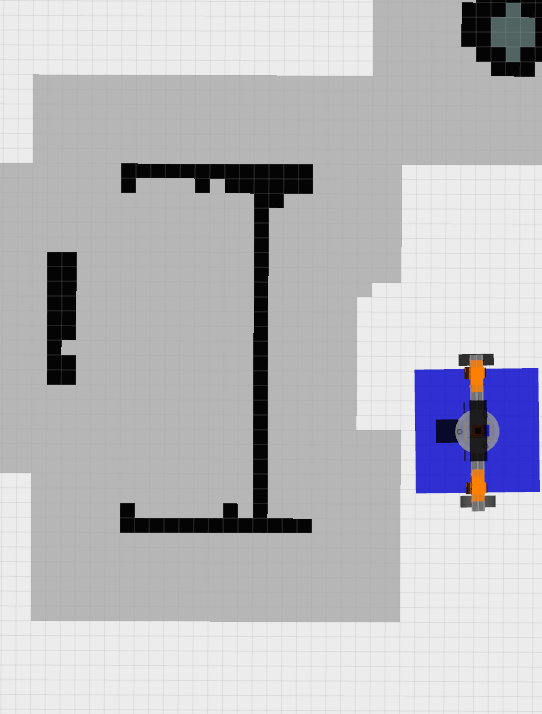
\includegraphics[width=0.45\textwidth]{Figures/InflationExample1.png}
        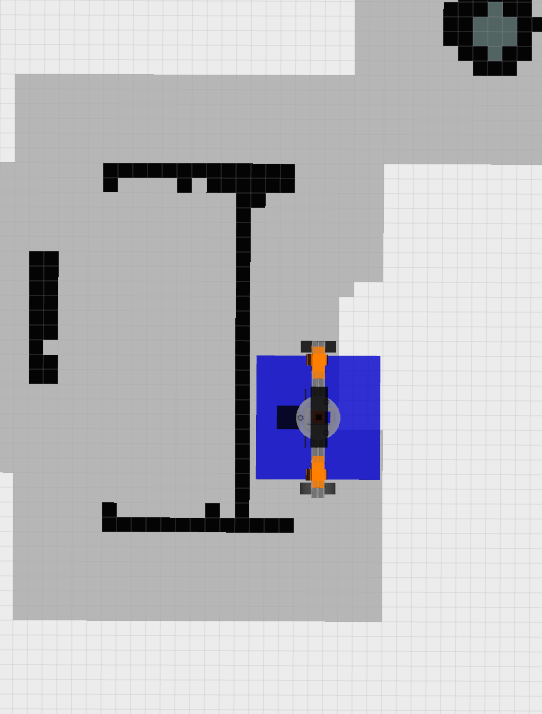
\includegraphics[width=0.45\textwidth]{Figures/InflationExample2.png}
      \end{figure}
    \end{column}
    \begin{column}{0.4\textwidth}
      \begin{itemize}
      \item Celdas blancas: espacio libre.
      \item Celdas negras: espacio con obstáculos.
        \item Celdas grises: espacio sin obstáculos donde el robot no puede estar debido a su tamaño. 
      \end{itemize}
    \end{column}
  \end{columns}
  \begin{itemize}
  \item Un mapa de celdas de ocupación debe \textit{inflarse} antes de usarse para planear rutas.
  \item Esta operación se conoce como \textit{dilatación} y es un operador morfológico como se verá en la sección de conceptos de visión.
  \item El inflado se usa para planeación de rutas, no para localización.
  \end{itemize}
\end{frame}

\begin{frame}\frametitle{Inflado de celdas de ocupación}
  \begin{algorithm}[H]
    \DontPrintSemicolon
    \KwData {\;
      Mapa $M$ de celdas de ocupación\;
      Radio de inflado $r_i$
    }
    \KwResult{Mapa inflado $M_{inf}$}
    $M_{inf} = $ Copia de $M$\;
    \ForEach{$i\in [0,\dots,rows)$}
      {
        \ForEach{$j\in [0,\dots,cols)$}
          {
            //Si la celda está ocupada, marcar como ocupadas las $r_i$ celdas de alrededor.\;
            \If{$M[i,j] == 100$ }
               {
                 \ForEach{$k_1\in [-r_i,\dots,r_i]$}
                   {
                     \ForEach{$k_2\in [-r_i,\dots,r_i]$}
                       {
                         $M_{inf}[i+k_1, j+k_2] = 100$
                       }
                   }
               }    
          }
        }
        \caption{Algoritmo de inflado de mapas}
  \end{algorithm}
\end{frame}

\begin{frame}[containsverbatim]\frametitle{Ejercicio 2 - Inflado de mapas}
  \begin{enumerate}
  \item Ejecute la simulación con el comando \texttt{roslaunch bring\_up path\_planning.launch}
  \item Ejecute el algoritmo de inflado de mapas \texttt{rosrun exercises map\_inflation.py}
  \item Mediante la GUI, modifique el valor de inflación en el campo correspondiente y observe los cambios en el visualizador RViz.
  \end{enumerate}
\end{frame}

\begin{frame}\frametitle{Mapas de líneas}
  También son mapas geométricos, pero al almacenar \textit{features} requieren mucho menos memoria. La desventaja es la dificultad para extraer líneas del ambiente y la poca precisión en el empatado. 
  \begin{figure}
    \centering
    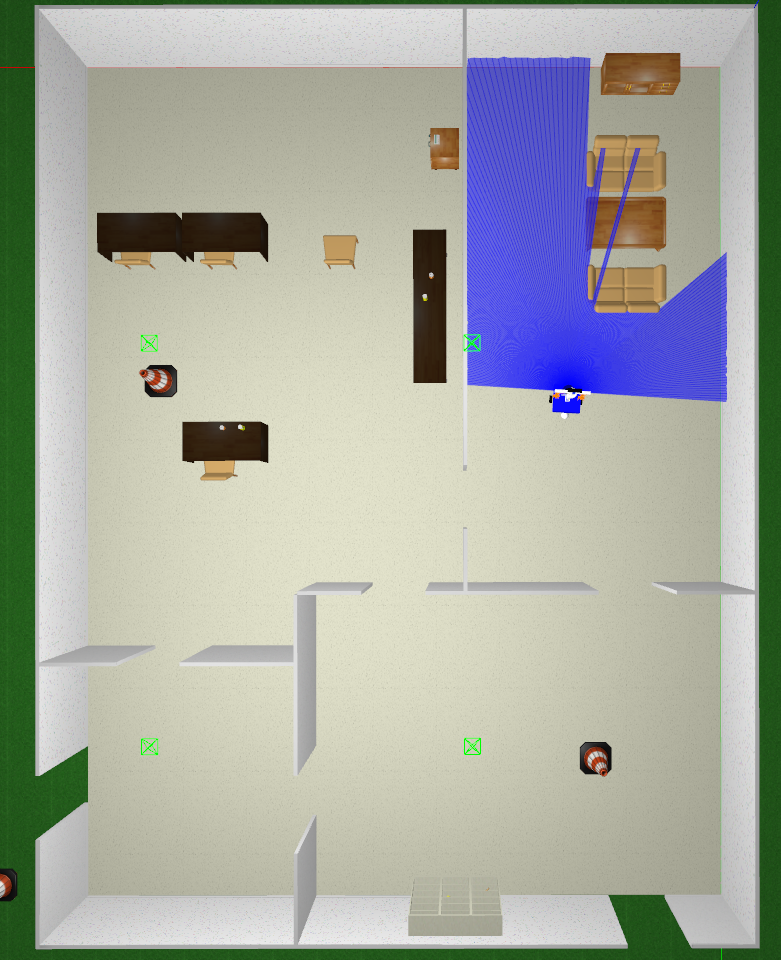
\includegraphics[width=0.3\textwidth]{Figures/MapLinesGazebo.png}
    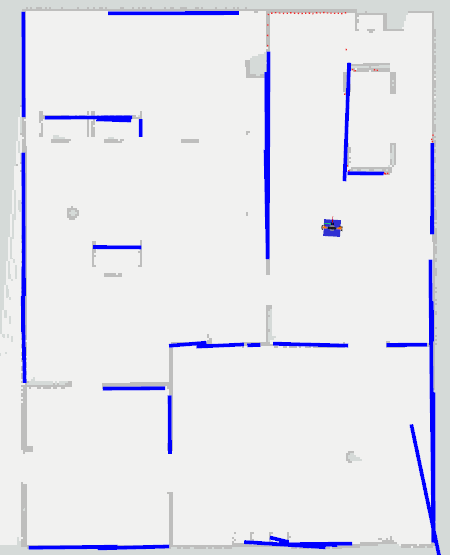
\includegraphics[width=0.3\textwidth]{Figures/MapLines.png}
  \end{figure}
  Algunos métodos para extraer líneas:
  \begin{itemize}
  \item \textit{Split and merge}
  \item Transformada Hough (se verá en la sección de visión computacional)
  \item RANSAC
  \end{itemize}
\end{frame}

\begin{frame}\frametitle{Algoritmo \textit{Split and Merge}}
  Se utiliza principalmente cuando los datos provienen de un sensor Lidar y por lo tanto, los puntos están en secuencia.
  \[\]
  \begin{columns}
    \begin{column}{0.65\textwidth}
      \begin{algorithm}[H]
        \DontPrintSemicolon
        \KwData {Conjunto de puntos $P$}
        \KwResult{Conjunto de líneas en forma normal $(\rho, \theta$)}
        \;
        Ajustar una recta $L$ al conjunto $P$ por mínimos cuadrados\;
        Encontrar el punto $p_i$ más lejano a la recta\;
          \uIf{$d(p_i, L) > umbral$}
             {
               Dividir $P$ en dos subconjuntos $P_1$ y $P_2$ usando $p_i$ como pivote\;
               Aplicar este algoritmo recursivamente para $P_1$ y $P_2$\;
               Devolver las rectas de ambos subconjuntos
             }
             \Else
                 {
                   Devolver la recta $L$ en forma normal $(\rho, \theta)$\;
                 }
                 \caption{\textit{Split and Merge}}
        \end{algorithm}
    \end{column}
    \begin{column}{0.35\textwidth}
      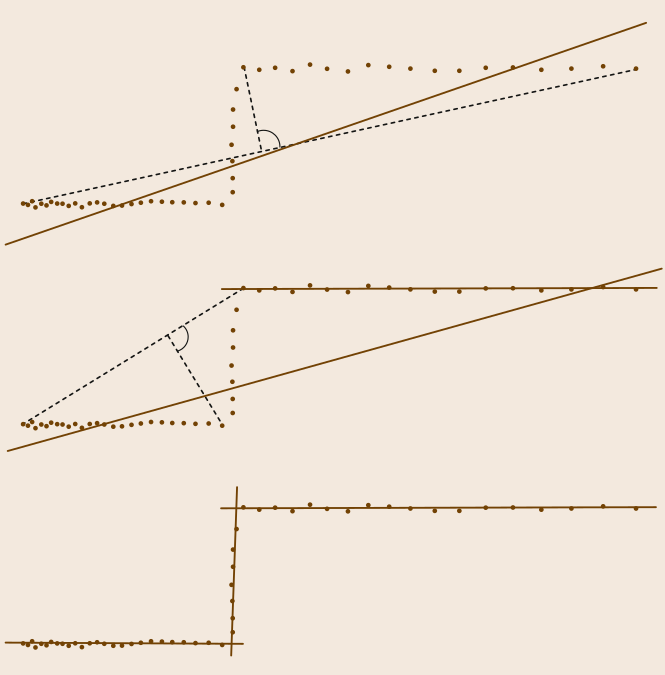
\includegraphics[width=\textwidth]{Figures/SplitAndMerge.png}
    \end{column}
  \end{columns}
\end{frame}

\begin{frame}\frametitle{Mínimos cuadrados}
  Este método busca minimizar las distancias entre los puntos $(x_i,y_i)$ y la recta en forma normal dada por los parámetros $(\rho, \theta)$.
  \[\]
  Dado un conjunto de puntos $(x_i, y_i)$, la recta $(\rho,\theta)$ que mejor se ajusta se puede obtener con:
  \begin{eqnarray*}
    \theta &=& \frac{1}{2}\atantwo\left(-2\sum_i (\bar{x} - x_i)(\bar{y}-y_i)\quad,\quad \sum_i\left[(\bar{y} - y_i)^2 - (\bar{x} - x_i)^2\right]\right)\\
    \rho &=& \bar{x}\cos\theta + \bar{y}\sin\theta
  \end{eqnarray*}
  con
  \begin{eqnarray*}
    \bar{x} &=& \frac{1}{n}\sum_i x_i\\
    \bar{y} &=& \frac{1}{n}\sum_i y_i
  \end{eqnarray*}
\end{frame}

\begin{frame}[containsverbatim]\frametitle{Ejercicio 3 - Mapas de líneas}
  \begin{enumerate}
  \item Ejecute la simulación con el comando \texttt{roslaunch bring\_up path\_planning.launch}
  \item Ejecute el algoritmo \textit{split and merge} con el comando: \texttt{rosrun exercises split\_and\_merge.py}
  \item Mediante la GUI, mueva el robot en el espacio libre y observe el desempeño del algoritmo
  \end{enumerate}
\end{frame}


\begin{frame}\frametitle{Diagrama de Voronoi Generalizado}
  \begin{itemize}
  \item A diferencia de los mapas geométricos, donde se busca reflejar la forma exacta del ambiente, los \textbf{mapas topológicos} buscan representar solo las relaciones espaciales de los puntos de interés.
  \item Los Diagramas de Voronoi dividen el espacio en regiones. Cada región está asociada a un punto llamado semilla, sitio o generador. Una región asociada a una semilla $x$ contiene todos los puntos $p$ tales que $d(x,p)$ es menor o igual que la distancia $d(x^\prime, p)$ a cualquier otra semilla $x^\prime$.
  \item Un diagrama de Voronoi generalizdo (GVD) considera que las semillas pueden ser objetos con dimensiones y no solo puntos. 
  \end{itemize}
  \begin{figure}
    \centering
    
\includegraphics[height=0.4\textheight]{Figures/GVD.png}
    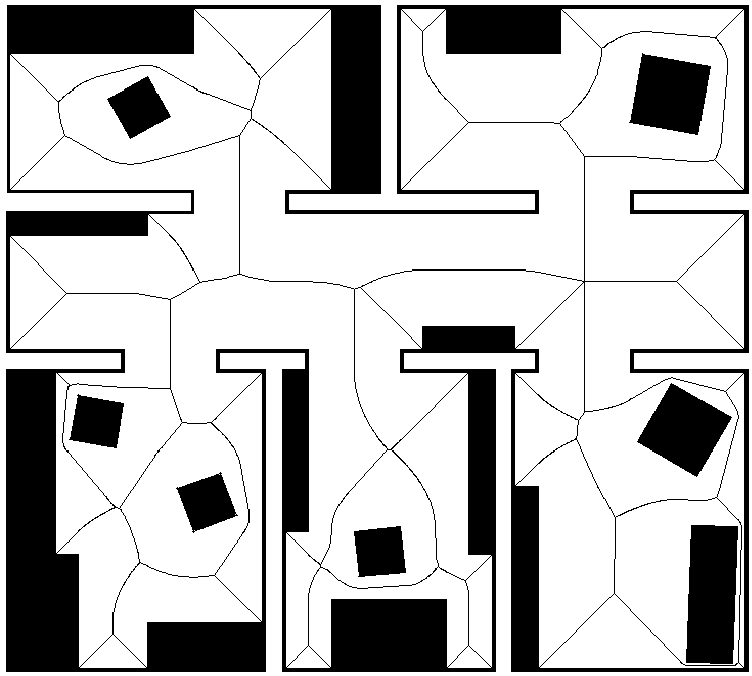
\includegraphics[height=0.4\textheight]{Figures/GVDExample.png}
  \end{figure}
  \begin{itemize}
    \item La forma de las regiones depende de la función de distancia que se utilice. 
  \end{itemize}
\end{frame}

\begin{frame}\frametitle{El algoritmo \textit{Brushfire}}
  \begin{columns}
    \begin{column}{0.65\textwidth}
      \begin{itemize}
      \item Obtener un GVD es aún un problema abierto
      \item Se simplifica el problema si se asume que el espacio está representado por Celdas de Ocupación
      \item En este caso el GVD se puede obtener mediante el algoritmo \textit{Brushfire}
      \item El mapa de rutas mostrado en la figura se forma con las celdas que son máximos locales en el mapa de distancias devuelto por Brushfire, es decir, son las celdas que son fronteras entre las regiones de Voronoi.
      \item Estas celdas también son aquellas equidistantes a los dos obstáculos más cercanos. 
      \end{itemize}
    \end{column}
    \begin{column}{0.35\textwidth}
      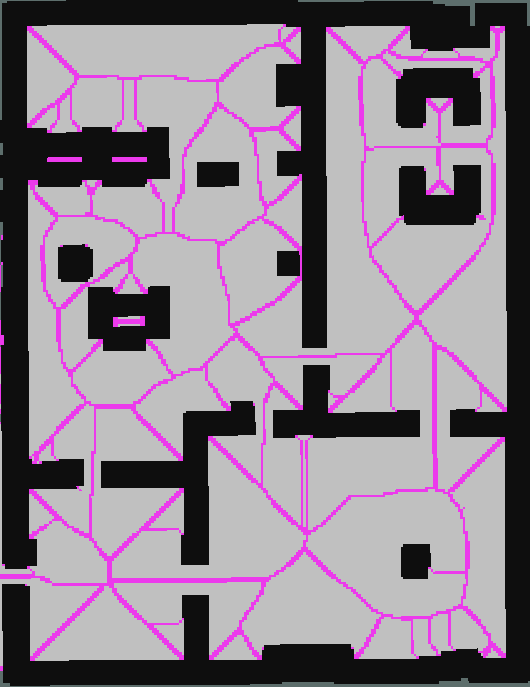
\includegraphics[width=\textwidth]{Figures/GVDFromGrid.png}
    \end{column}
  \end{columns}
\end{frame}

\begin{frame}\frametitle{El algoritmo \textit{Brushfire}}
  \begin{columns}
    \begin{column}{0.65\textwidth}
      \begin{algorithm}[H]
        \DontPrintSemicolon
        \KwData {Mapa de celdas de ocupación $M$}
        \KwResult{Distancias de cada celda al objeto más cercano}
        \;
        Fijar $d(p) = 0$ para toda celda $p$ en los obstáculos\;
        Fijar $d(p) = -1$ para toda celda $p$ en el espacio libre\;
        Crear una cola $Q$ y agregar toda $p$ en los obstáculos\;
        \While{$Q$ no esté vacía}
              {
                $x = $ desencolar de Q\;
                \ForAll{celdas $p$ vecinas de $x$}
                       {
                         \uIf{$d(p) == -1$}
                            {
                              Agregar $p$ a $Q$\;
                              Fijar $d(p) = x + d(p,x)$\;
                            }
                            \Else
                                {
                                  Fijar $d(p) = min(d(p), x+d(p,x))$
                                }
                       }
              }
        \caption{Brushfire}
        \end{algorithm}
    \end{column}
    \begin{column}{0.35\textwidth}
      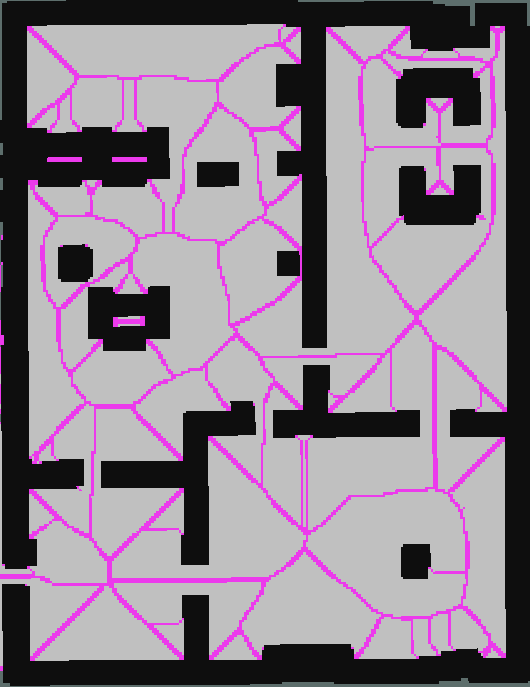
\includegraphics[width=\textwidth]{Figures/GVDFromGrid.png}
    \end{column}
  \end{columns}
\end{frame}

\begin{frame}[containsverbatim]\frametitle{Ejercicio 4 - Diagrama de Voronoi Generalizado}
  \begin{enumerate}
  \item Ejecute la simulación con el comando \texttt{roslaunch bring\_up path\_planning.launch}
  \item Ejecute el inflado de mapas: \texttt{rosrun exercises map\_inflation.py}
  \item Ejecute el algoritmo de \texttt{brushfire} mediante el comando \texttt{rosrun exercises voronoi.py}
  \item Observe el diagrama resultante en el visualizador RViz.
  \end{enumerate}
\end{frame}

\begin{frame}\frametitle{Planeación de rutas}
  La planeación de rutas consiste en encontrar una secuencia de puntos $q\in Q_{free}$ que permitan al robot moverse desde una configuración inicial $q_{start}$ hasta una configuración final $q_{goal}$.
  \begin{itemize}
  \item Una \textbf{ruta} es solo la secuencia de configuraciones para llegar a la meta.
  \item Cuando la secuencia de configuraciones se expresa en función del tiempo, entonces se tiene una \textbf{trayectoria}. 
  \end{itemize}
  En este curso solo vamos a hacer planeación de rutas, no de trayectorias (para navegación).\\
  Existen varios métodos para planear rutas. La mayoría de ellos se pueden agrupar en:
  \begin{itemize}
  \item Métodos basados en muestreo
  \item Métodos basados en grafos
  \end{itemize}
\end{frame}

\begin{frame}\frametitle{Métodos basados muestreo}
  Como su nombre lo indica, consisten en tomar muestras aleatorias del espacio libre. Si es posible llegar en línea recta de la configuración actual al punto muestrado, entonces se agrega a la ruta.
  Ejemplos:
  \begin{itemize}
  \item RRT (Rapidly-exploring Random Trees)
  \item RRT-Bidireccional
  \item RRT-Extendido
  \end{itemize}
\end{frame}

\begin{frame}\frametitle{\textit{Rapidly-exploring Random Trees}}
  Consiste en construir un árbol a partir de muestras aleatorias del espacio libre.
  \begin{columns}
    \begin{column}{0.4\textwidth}
      \begin{algorithm}[H]\small
        \KwData{Mapa, $q_{s} = $ Punto origen }
        \KwResult{Espacio explorado}
        Árbol[0] = $q_{s}$\;
        $k$ = 0\;
        \While{$k < k_{max}$ }
              {
                $q_{r}$ = ConfiguracionAleaoria()\;
                Extiende(Árbol, $q_{r}$)\;
                $k++$\;
              }
              \Return Árbol\;
              \caption{RRT}
      \end{algorithm}
    \end{column}
    \begin{column}{0.6\textwidth}
      \begin{figure}
        \centering
        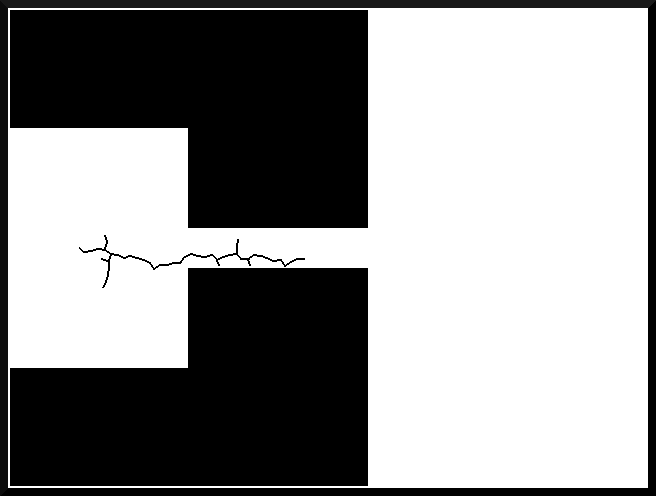
\includegraphics[width=0.45\textwidth]{Figures/RRTO010.png}
        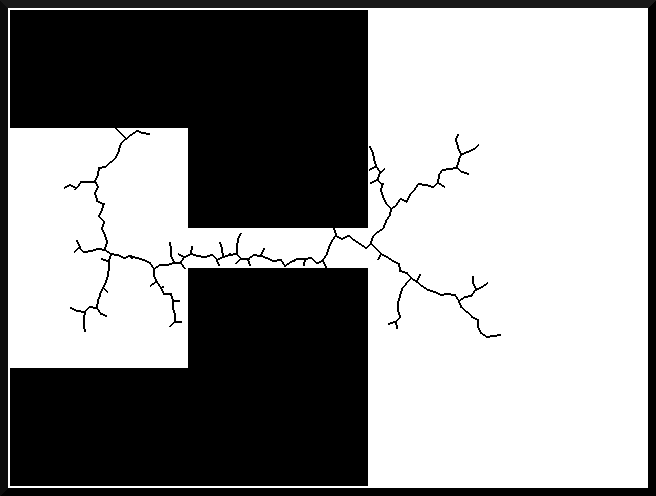
\includegraphics[width=0.45\textwidth]{Figures/RRTO0100.png}
        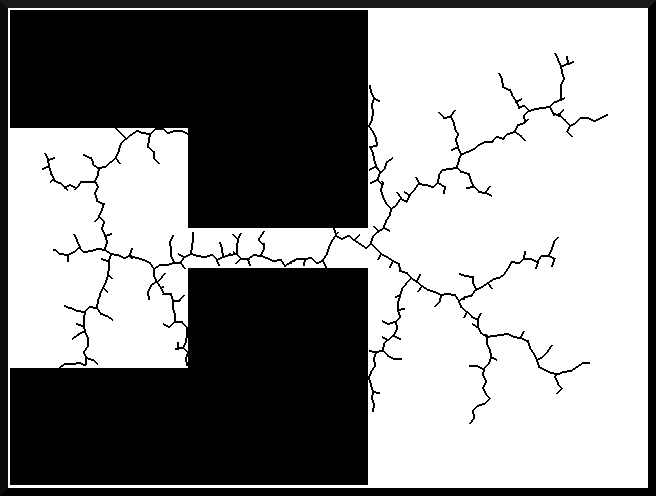
\includegraphics[width=0.45\textwidth]{Figures/RRTO0300.png}
      \end{figure}
    \end{column}
  \end{columns}
\end{frame}

\begin{frame}\frametitle{Métodos basados en grafos}
  Estos métodos consideran el ambiente como un grafo. En el caso de celdas de ocupación, cada celda libre es un nodo que está conectado con las celdas vecinas que también estén libres. Los pasos generales de este tipo de algorimos se pueden resumir en:
  \[\]
  \begin{algorithm}[H]
    \footnotesize
    \DontPrintSemicolon
    \KwData {Mapa $M$ de celdas de ocupación, configuración inicial $q_{start}$, configuración meta $q_{goal}$}
    \KwResult{Ruta $P=[q_{start},q_1, q_2, \dots , q_{goal}]$}
    Obtener los nodos $n_s$ y $n_g$ correspondientes a $q_{start}$ y $q_{goal}$\;
    Lista abierta $OL = \emptyset$ y lista cerrada $CL = \emptyset$\;
    Agregar $n_s$ a $OL$\;
    Nodo actual $n_c = n_s$\;
    \While{$OL\neq \emptyset$ y $n_c\neq n_g$}
    {
      Seleccionar $n_c$ de $OL$ \textbf{bajo algún criterio}\;
      Agregar $n_c$ a $CL$\;
      Expandir $n_c$\;
      Agregar a $OL$ los vecinos de $n_c$ que no estén ya en $OL$ ni en $CL$\;
    }
    \If{$n_c\neq n_g$}{Anunciar Falla}
    Obtener la configuración $q_i$ para cada nodo $n_i$ de la ruta\;
  \end{algorithm}
\end{frame}

\begin{frame}\frametitle{Métodos basados en grafos}
  El criterio para seleccionar el siguiente nodo a expandir $n_c$ de la lista abierta, determina el tipo de algoritmo:
  \begin{itemize}
  \item Criterio FIFO: Búsqueda a lo ancho BFS (la lista abierta es una cola)
  \item Criterio LIFO:  Búsqueda en profundidad DFS (la lista abierta es una pila)
  \item Menor valor $g$: Dijkstra (la lista abierta es una cola con prioridad)
  \item Menor valor $f$: A* (la lista abierta es una cola con prioridad)
  \end{itemize}
  Si el costo $g$ para ir de una celda a otra es siempre 1, entonces Dijkstra es equivalente a BFS. \\
  A* y Dijkstra siempre calculan la misma ruta pero A* lo hace más rápido. 
\end{frame}

\begin{frame}\frametitle{Mapas de costo}
  \begin{itemize}
  \item Los métodos como Dijkstra y A* minimizan una función de costo. Esta función podría ser distancia, tiempo de recorrido, número de vuelta, energía gastada, entre otras.
  \item En este curso se empleará como costo una combinación de distancia recorrida más peligro de colisión (cercanía a los obstáculos).
  \item De este modo, las rutas serán un equilibrio entre rutas cortas y rutas seguras.
  \end{itemize}
  \begin{figure}
    \centering
    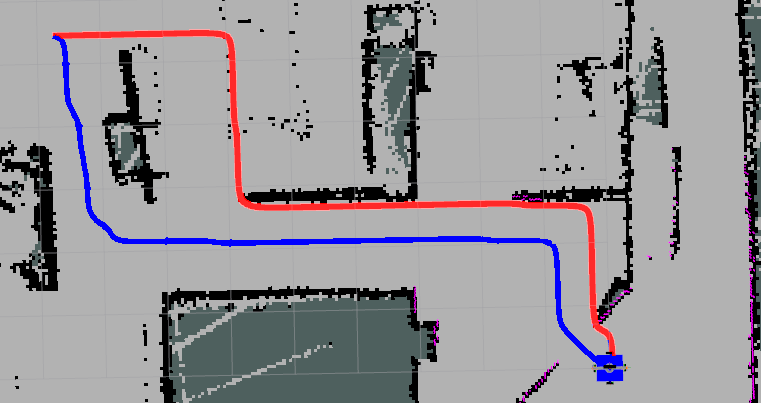
\includegraphics[width=0.5\textwidth]{Figures/AStarComparison.png}
  \end{figure}
\end{frame}

\begin{frame}\frametitle{Mapas de costo}
  \begin{itemize}
  \item Se utilizará como costo una función de \textit{cercanía}.
  \item Se calcula de forma similar al algoritmo Brushfire, pero la función decrece conforme nos alejamos de los objetos. 
  \end{itemize}
  \begin{columns}
    \begin{column}{0.6\textwidth}
      \begin{algorithm}[H]
        \footnotesize
        \DontPrintSemicolon
        \KwData {\;
          Mapa $M$ de celdas de ocupación\;
          Radio de costo $r_c$
        }
        \KwResult{Mapa de costo $M_c$}
        \;
        $M_c = $ Copia de $M$\;
        \ForEach{$i\in [0,\dots,rows)$}
          {
            \ForEach{$j\in [0,\dots,cols)$}
              {
                //Si está ocupada, calcular el costo de $r_c$ celdas alrededor.\;
                \If{$M[i,j] == 100$ }
                   {
                     \ForEach{$k_1\in [-r_c,\dots,r_c]$}
                             {
                               \ForEach{$k_2\in [-r_c,\dots,r_c]$}
                                       {
                                         $C = r_c - max(|k1|,|k2|) + 1$\;
			                 $M_c[i+k1,j+k2] = max(C, M_c[i+k1,j+k2]$\;
                                       }
                             }
                   }    
              }
            }
            \caption{Mapa de costo}
      \end{algorithm}
    \end{column}
    \begin{column}{0.4\textwidth}
      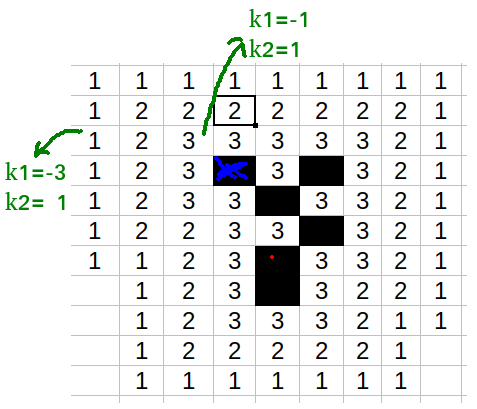
\includegraphics[width=0.95\textwidth]{Figures/CostMap.png}
    \end{column}
  \end{columns}
\end{frame}

\begin{frame}\frametitle{El algoritmo A*}
  \begin{itemize}
  \item Es un algoritmo completo, es decir, si la ruta existe, seguro la encontrará, y si no existe, lo indicará en tiempo finito.
  \item Al igual que Dijkstra, A* encuentra una ruta que minimiza una función de costo, es decir, es un algoritmo óptimo.
  \item Es un algoritmo del tipo de búsqueda informada, es decir, utiliza información sobre el estimado del costo restante para llegar a la meta para priorizar la expansión de ciertos nodos. 
  \item El nodo a expandir se selecciona de acuerdo con la función:
    \[f(n) = g(n) + h(n)\]
    donde
    \begin{itemize}
    \item $g(n)$ es el costo acumulado del nodo $n$
    \item $h(n)$ es una función heurística que \textbf{subestima} el costo de llegar del nodo $n$ al nodo meta $n_g$. 
    \end{itemize}
  \item Se tienen los siguientes conjuntos importantes:
    \begin{itemize}
    \item Lista abierta: conjunto de todos los nodos en la frontera (visitados pero no conocidos). Es una cola con prioridad donde los elementos son los nodos y la prioridad es el valor $f(n)$.
    \item Lista cerrada: conjunto de nodos para los cuales se ha calculado una ruta óptima. 
    \end{itemize}
    \item A cada nodo se asocia un valor $g(n)$, un valor $f(n)$ y un nodo padre $p(n)$. 
  \end{itemize}
\end{frame}

\begin{frame}\frametitle{El algoritmo A*}
    \begin{algorithm}[H]
    \footnotesize
    \DontPrintSemicolon
    \KwData {Mapa $M$, nodo inicial $n_s$ con configuración $q_{s}$, nodo meta $n_g$ con configuración $q_{g}$}
    \KwResult{Ruta óptima $P=[q_{s},q_1, q_2, \dots , q_{g}]$}
    Lista abierta $OL = \emptyset$ y lista cerrada $CL = \emptyset$\;
    Fijar $f(n_{s}) = 0$, $g(n_{s}) = 0$ y $prev(n_{s}) = NULL$\;
    Agregar $n_s$ a $OL$ y fijar nodo actual $n_c = n_s$\;
    \While{$OL\neq \emptyset$ y $n_c\neq n_g$}
    {
      Remover de $OL$ el nodo $n_c$ con el menor valor $f$ y agregar $n_c$ a $CL$\;
      \ForAll{$n$ vecino de $n_c$}
             {
               $g = g(n_c) + costo(n_c, n)$\;
               \If{$g < g(n)$}
                  {
                    $g(n) = g$\;
                    $f(n) = h(n) + g(n)$\;
                    $prev(n) = n_c$\;
                  }
             }
      Agregar a $OL$ los vecinos de $n_c$ que no estén ya en $OL$ ni en $CL$\;
    }
    \If{$n_c\neq n_g$}{Anunciar Falla}
    \While{$n_c \neq NULL$}
          {
            Insertar al inicio de la ruta $P$ la configuración correspondiente al nodo $n_c$\;
            $n_c = prev(n_c)$
          }
    Devolver ruta óptima $P$
  \end{algorithm}
\end{frame}

\begin{frame}\frametitle{El algoritmo A*}
  \begin{itemize}
  \item La función de costo será el número de celdas más el mapa de costo de la clase anterior.
  \item Puesto que el mapa está compuesto por celdas de ocupación, los nodos vecinos se pueden obtener usando conectividad 4 o conectividad 8.
  \item Si se utiliza conectividad 4, la distancia de Manhattan es una buena heurística.
  \item Si se utiliza conectividad 8, se debe usar la distancia Euclideana.
  \item La lista abierta se puede implementar con una \textit{Heap}, de este modo, la inserción de los nodos $n$ se puede hacer en tiempo logarítmico y la selección del nodo con menor $f$ se hace en tiempo constante.
  \item La obtención de las coordenadas $(x,y)$ a partir de los nodos $n$ se puede hacer con:
    \begin{eqnarray*}
      x &=& (c)\delta + M_{ox}\\
      y &=& (r)\delta + M_{oy}
    \end{eqnarray*}
  \item La obtención del renglón-columna $(r,c)$ del nodo $n$ a partir de $(x,y)$, se puede obtener con:
    \begin{eqnarray*}
      r &=& int((y - M_{oy})/\delta)\\
      c &=& int((x - M_{ox})/\delta)
    \end{eqnarray*}
    donde
    \begin{itemize}
    \item $(M_{ox}, M_{oy})$ es el origen del mapa, es decir, las coordenadas cartesianas de la celda (0,0).
    \item $\delta$ es la resolución, es decir, el tamaño de cada celda.
    \item La función $int()$ convierte a entero el argumento. 
    \end{itemize}
    \item Todos estos valores están en los metadatos del mapa. 
  \end{itemize}
\end{frame}

\begin{frame}\frametitle{El algoritmo A*}
  Ejemplo: ¿Cuál es la ruta óptima del nodo A al nodo Z?
  \begin{figure}
    \centering
    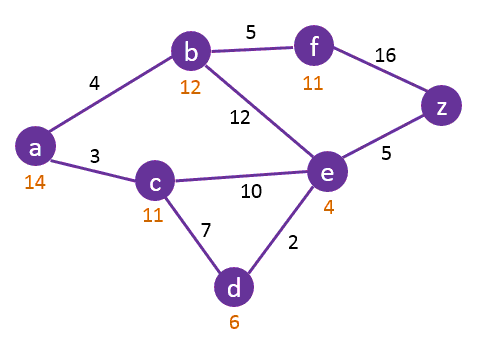
\includegraphics[width=0.5\textwidth]{Figures/AStarExample.png}
  \end{figure}
\end{frame}

\begin{frame}\frametitle{El algoritmo A*}
  \begin{table}
    \begin{tabular}{cccc}
      Paso & Nodo actual & Lista Cerrada & Lista abierta\\
      \hline
      0   & NULL & $\emptyset$          & \{A\}      \\
      1   & A    & \{A\}                & \{B, C\}   \\
      2   & C    & \{A, C\}             & \{B, D, E\}\\
      3   & B    & \{A, C, B\}          & \{D, E, F\}\\
      4   & D    & \{A, C, B, D\}       & \{E, F\}   \\
      5   & $E$  & \{A, C, B, D, E\}    & \{F, Z\}   \\
      6   & $Z$  & \{A, C, B, D, E, Z\} & \{F \}     \\
    \end{tabular}
  \end{table}
  \begin{table}
    \footnotesize
    \begin{tabular}{ccccccc}
      A & B & C & D & E & F & Z \\
      g,f,p & g,f,p & g,f,p & g,f,p & g,f,p & g,f,p & g,f,p\\
      \hline
      0,0,NULL & $\infty,\infty$,NULL & $\infty,\infty$,NULL & $\infty,\infty$,NULL & $\infty,\infty$,NULL & $\infty,\infty$,NULL & $\infty,\infty$,NULL\\
      0,0,NULL & 4, 16, A             & 3, 14, A             & $\infty,\infty$,NULL & $\infty,\infty$,NULL & $\infty,\infty$,NULL & $\infty,\infty$,NULL\\
      0,0,NULL & 4, 16, A             & 3, 14, A             & 10, 16, C            & 13, 17, C            & $\infty,\infty$,NULL & $\infty,\infty$,NULL\\
      0,0,NULL & 4, 16, A             & 3, 14, A             & 10, 16, C            & 13, 17, C            & 9, 20, B             & $\infty,\infty$,NULL\\
      0,0,NULL & 4, 16, A             & 3, 14, A             & 10, 16, C            & \textbf{12, 16, D}   & 9, 20, B             & $\infty,\infty$,NULL\\
      0,0,NULL & 4, 16, A             & 3, 14, A             & 10, 16, C            &         12, 16, D    & 9, 20, B             & 17, 17, E           \\
      0,0,NULL & 4, 16, A             & 3, 14, A             & 10, 16, C            &         12, 16, D    & 9, 20, B             & 17, 17, E           \\
    \end{tabular}
  \end{table}
\end{frame}

\begin{frame}[containsverbatim]\frametitle{Ejercicio 5 - Planeación de rutas}
  \begin{enumerate}
  \item Ejecute la simulación con el comando \texttt{roslaunch bring\_up path\_planning.launch}
  \item Ejecute el algoritmo de inflado de mapas \texttt{rosrun exercises map\_inflation.py}
  \item Ejecute el cálculo de mapas de costo \texttt{rosrun exercises map\_cost}
  \item Ejecute el algoritmo A* \texttt{rosrun exercises a\_star.py}
  \item Mediante la GUI, fije un punto meta y observe la ruta calculada en el visualizador RViz.
  \item Detenga el nodo de A*
  \item Abra el archivo \texttt{catkin\_ws/src/exercises/scripts/a\_start.py}, comente la línea 43 y descomente la línea 44.
  \item Ejecute nuevamente el algoritmo A*
  \item Fije un punto meta mediante la GUI y observe los cambios en las rutas calculadas.
  \end{enumerate}
\end{frame}

\begin{frame}\frametitle{Seguimiento de rutas}
  Hasta el momento ya se tiene una representación del ambiente y una forma de planear rutas. Ahora falta diseñar las leyes de control que hagan que el robot se mueva por la ruta calculada. Este control se hará bajo los siguientes supuestos:
  \begin{itemize}
  \item Se conoce la posición del robot (más adelante se abodará el problema de la localización)
  \item El modelo cinemático es suficiente para modelar el movimiento del robot 
  \item Las dinámicas no modeladas (parte eléctrica y mecánica de los motores) son lo suficientemente rápidas para poder despreciarse
  \end{itemize}
\end{frame}

\begin{frame}\frametitle{Modelo cinemático}
  Considere la base móvil omnidireccional de la figura con configuración $q=(x,y,\theta)$.
  \begin{columns}
    \begin{column}{0.5\textwidth}
      \begin{figure}
        \centering
        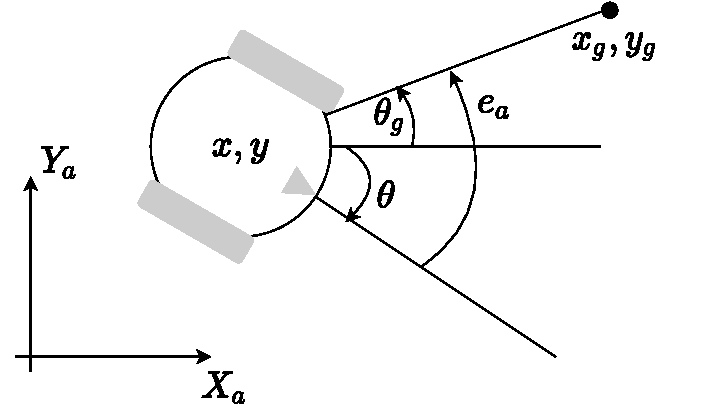
\includegraphics[width=\textwidth]{Figures/GoalPose.pdf}
      \end{figure}
    \end{column}
    \begin{column}{0.5\textwidth}
      El modelo cinemático está dado por
      \begin{eqnarray*} 
        \dot{x} &=& v_x\cos\theta - v_y\sin\theta\label{eq:Kinematic1}\\         
        \dot{y} &=& v_x\sin\theta + v_y\cos\theta\\ 
        \dot{\theta} &=& \omega,\label{eq:Kinematic3}
      \end{eqnarray*}
    \end{column}
  \end{columns}
  \[\]
  \begin{itemize}
  \item $(v_x, v_y, \omega)$ se consideran como señales de control
  \item Corresponden a las velocidades lineales frontal y lateral, y la velocidad angular, con respecto al robot.
  \item La forma de convertir $(v_x, v_y, \omega)$ a velocidades de cada motor varía dependiendo del número de motores y de su posición. 
  \end{itemize}
\end{frame}

\begin{frame}\frametitle{Control de posición}
  \begin{itemize}
  \item Las leyes de control se diseñarán considerando una base diferencial
  \item Es mejor mover al robot así, pues lo sensores están generalmente al frente
  \end{itemize}
  Si se quiere alcanzar el punto meta $(x_g, y_g)$, las siguientes leyes de control siguientes permiten alcanzar dicho punto meta:
  \begin{eqnarray*}
  v_x    &=& v_{max}e^{-\frac{e_{\theta}^{2}}{\alpha}}\label{eq:Control11}\\
  \omega &=& \omega_{max}\left(\frac{2}{1+e^{-\frac{e_{\theta}}{\beta}}}-1\right)\label{eq:Control12}
  \end{eqnarray*}
  con
  \[e_{\theta} = \atantwo\left(y_g - y, x_g - x\right) - \theta\]
  El error de ángulo $e_\theta$ debe estar siempre en el intervalo $(-\pi, \pi]$. Si la diferencia resulta en un valor fuera de este ángulo, se puede acotar mediante:
  \[e_\theta \leftarrow \left(e_\theta + \pi\right)\% (2\pi) - \pi\]
  donde \% denota el operador módulo (residuo). 
\end{frame}

\begin{frame}\frametitle{Control de posición}
  \begin{itemize}
  \item $v_{max}$ y $\omega_{max}$ son las veloicidades linear y angular máximas y dependen de las capacidades físicas del robot.
  \item $\alpha$ y $\beta$ determinan qué tan rápido varían dichas velocidades cuando cambia el error de ángulo.
  \item En general, valores pequeños de $\alpha$ y $\beta$ logran que el robot alcance el punto meta casi en línea recta, sin embargo, valores muy pequeños pueden producir oscilaciones.
  \item Valores grandes de $\alpha$ y $\beta$ producen un movimiento más suave pero puede hacer que el robot describa curvas muy extensas. 
  \end{itemize}
  \begin{figure}
    \centering
    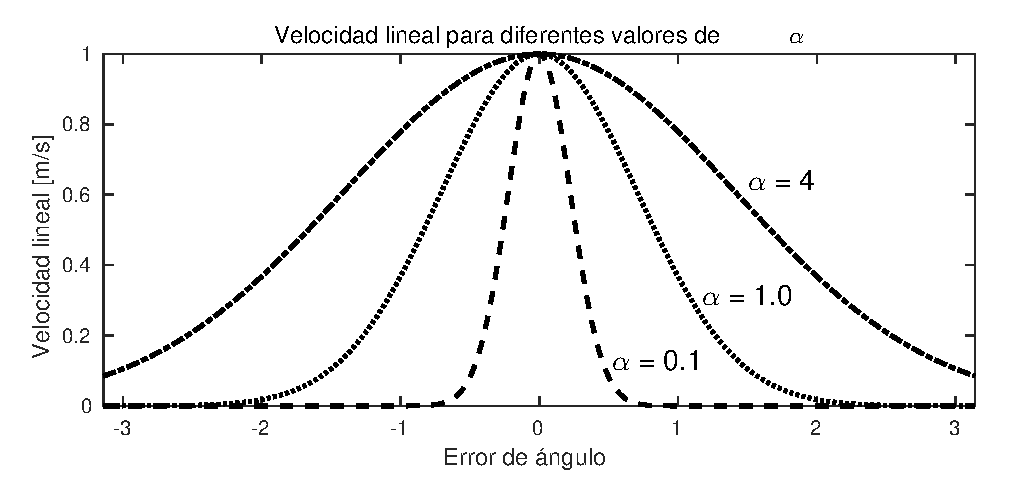
\includegraphics[width=0.45\textwidth]{Figures/LinearSpeed.eps}
    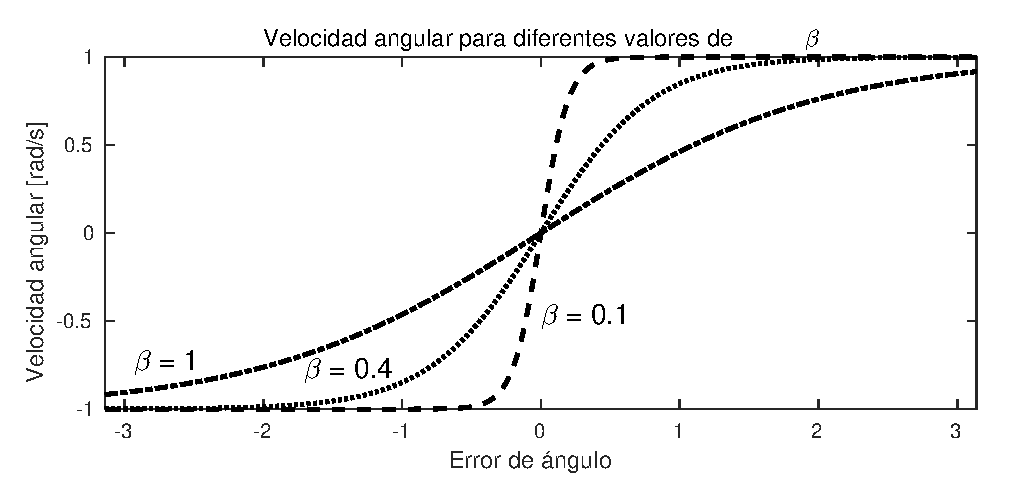
\includegraphics[width=0.45\textwidth]{Figures/AngularSpeed.eps}
  \end{figure}
\end{frame}

\begin{frame}\frametitle{Seguimiento de rutas}
  \begin{itemize}
  \item Hasta el momento se ha planteado cómo alcanzar una posición, pero, ¿para una ruta?
  \item Las rutas son secuencias de puntos. Esta secuencia se prodría parametrizar con respecto al tiempo para tener una trayectoria, sin embargo esto resulta muy complicado debido a la complejidad de las rutas.
  \item Una solución más sencilla es aplicar el control de posición para cada punto hasta recorrer toda la ruta.
  \item Las leyes de control solo dependen de $e_\theta$ por lo que el robot no desacelera al acercarse a la meta, provocando fuertes oscilaciones.
  \item Una forma de resolver este problema es ejecutar la ley de control sólo si la distancia al punto meta 

    \[d=\sqrt{(x_g - x_r)^2 + (y_g - y_r)^2}\] 
    
    es mayor que una tolerancia $\epsilon$.
  \item En este caso, el robot se detendrá abruptamente cuando el error de distancia sea menor que $\epsilon$, lo cual tampoco es deseable
  \item Una forma fácil de hacer que el robot acelere y desacelere, o en general, obtener un perfil de velocidad, es mediante el uso de una máquina de estados
    
  \end{itemize}
\end{frame}

\begin{frame}\frametitle{Perfil de velocidad}
  \begin{columns}
    \begin{column}{0.43\textwidth}
      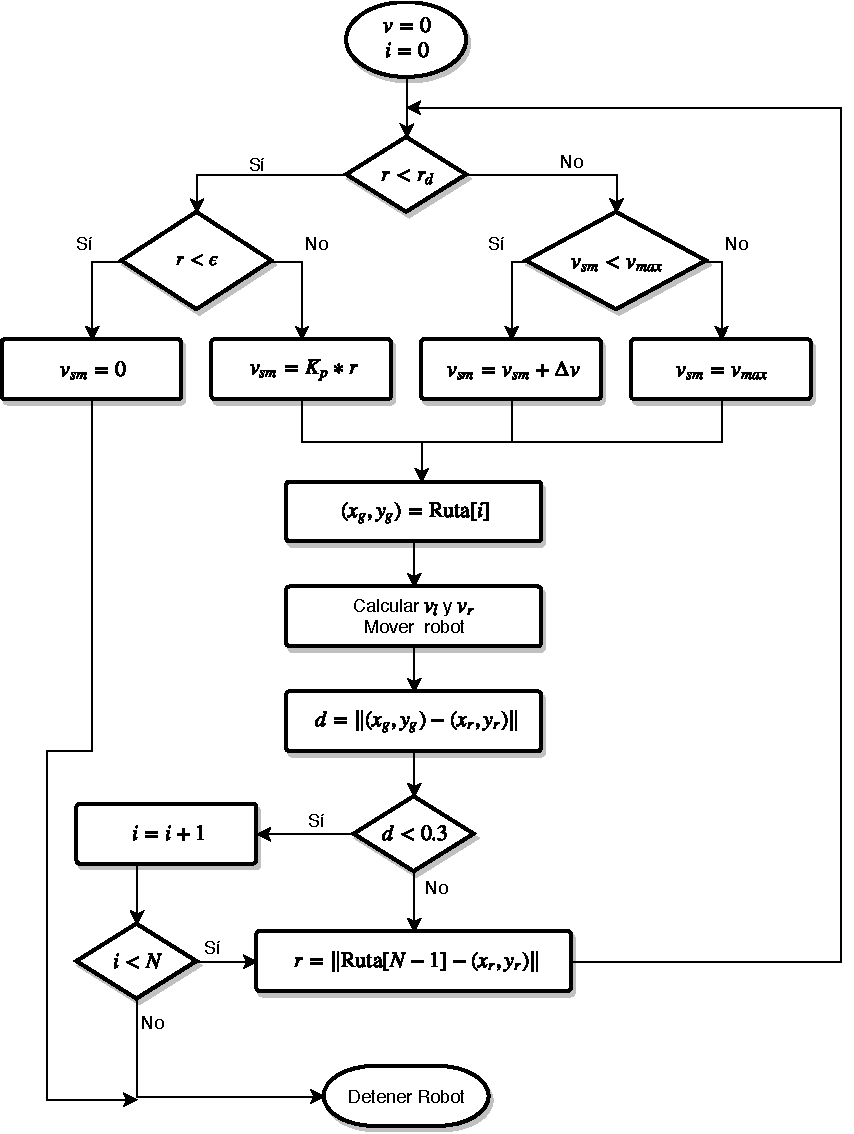
\includegraphics[width=\textwidth]{Figures/AFSM.pdf}
    \end{column}
    \begin{column}{0.5\textwidth}
      Considere una máquina de estados que calcule $v_{max}$ en el control. Sea $v_{sm}$ la nueva velocidad lineal máxima, de modo que ahora se tiene:
      \begin{eqnarray*}
        v      &=& v_{sm}e^{-\frac{e_{\theta}^{2}}{\alpha}}\label{eq:NewControl1}\\
        \omega &=& \omega_{max}\left(\frac{2}{1+e^{-\frac{e_{\theta}}{\beta}}}-1\right)\label{eq:NewControl2}
      \end{eqnarray*}
      con
      \begin{itemize}
      \item $r$: Distancia a la meta global
      \item $\epsilon$: Distancia a la que se considera que el robot alcanzó la meta global
      \item $r_d$: Distancia a la meta global para desacelerar
      \item $\Delta v$: Aceleración 
      \end{itemize}
    \end{column}
  \end{columns}
\end{frame}

\begin{frame}\frametitle{Perfil de velocidad}
  La siguiente figura muestra un ejemplo de una ruta y las velocidades lineales generadas usando solo las leyes de control (izquierda) y usando la máquina de estados para un perfil de velocidad (derecha). 
  \begin{figure}
    \centering
    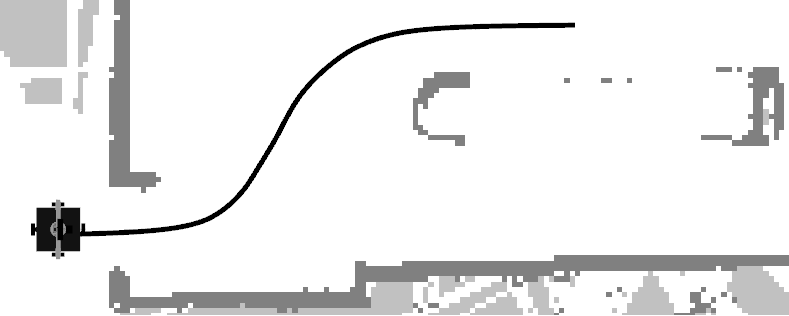
\includegraphics[width=0.45\textwidth]{Figures/SpeedProfilePath.png}
  \end{figure}
  \begin{figure}
    \centering
    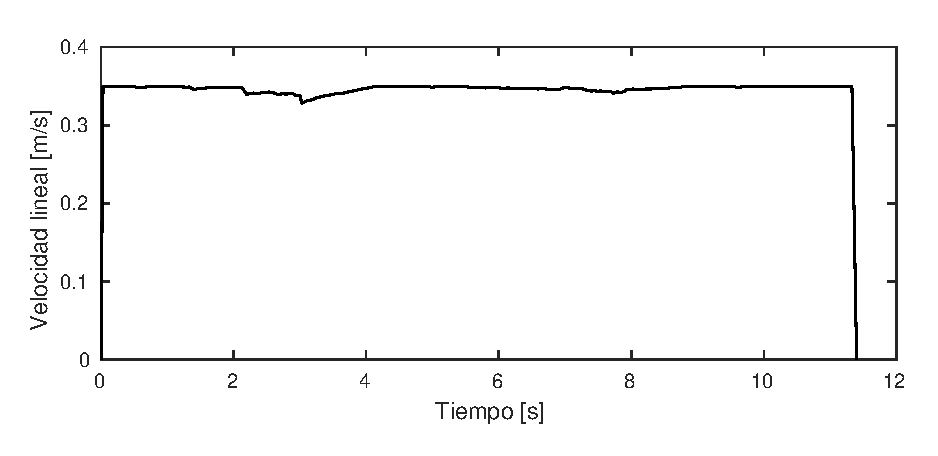
\includegraphics[width=0.45\textwidth]{Figures/SpeedWithoutProfile.eps}
    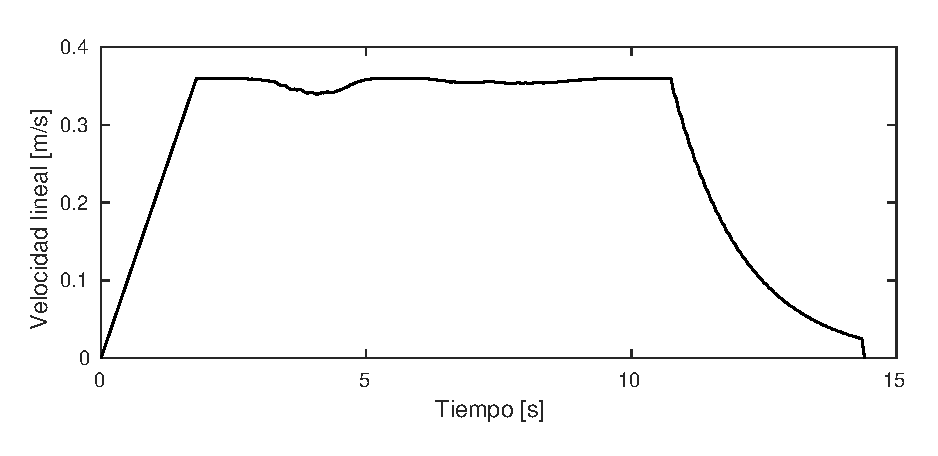
\includegraphics[width=0.45\textwidth]{Figures/SpeedWithProfile.eps}
  \end{figure}
\end{frame}

\begin{frame}[containsverbatim]\frametitle{Ejercicio 6 - Seguimiento de rutas}
  \begin{enumerate}
  \item Ejecute la simulación, el inflado de mapas, mapas de costo, el algoritmo A* y el control con el comando \texttt{roslaunch bring\_up navigation.launch}
  \item En el simulador RViz, con el botón ``2D Nav Goal'', indique una posición meta y observe el comportamiento. 
  \end{enumerate}
\end{frame}

\begin{frame}\frametitle{Evasión de obstáculos}
  \begin{itemize}
  \item Hasta el momento se tiene una manera de representar el ambiente, planear una ruta y seguirla
  \item ¿Qué pasa si en el ambiente hay un obstáculo que no estaba en el mapa?
  \item Se requiere de una técnica reactiva para evadir obstáculos
  \item Una posible solución es el uso de campos potenciales artificiales
  \end{itemize}
\end{frame}

\begin{frame}\frametitle{Campos potenciales artificiales}
  El objetivo de esta técnica es diseñar una función $U(q):\mathbb{R}^n\rightarrow \mathbb{R}$ que represente energía potencial.
  \begin{itemize}
  \item El gradiente $\nabla U(q) = \left[\frac{\partial U}{\partial q_1},\dots,\frac{\partial U}{\partial q_n}\right]$ es una fuerza.
  \item Se debe diseñar de modo que tenga un mínimo global en el punto meta y máximos locales en cada obstáculo.
  \item Si el robot se mueve siempre en sentido contrario al gradiente $\nabla U$ llegará al punto meta siguiendo una ruta alejada de los obstáculos.
  \item Ha varias formas de diseñar la función $U(q)$, algunas son:
    \begin{itemize}
    \item Algoritmo \textit{wavefront}, requiere una discretización del espacio (requiere mapa previo), pero no presenta mínimos locales.
    \item Campos atractivos y repulsivos, no requieren mapa previo, pero pueden presentar mínimos locales. 
    \end{itemize}
  \end{itemize}
\end{frame}

\begin{frame}\frametitle{Potenciales atractivos y repulsivos}
  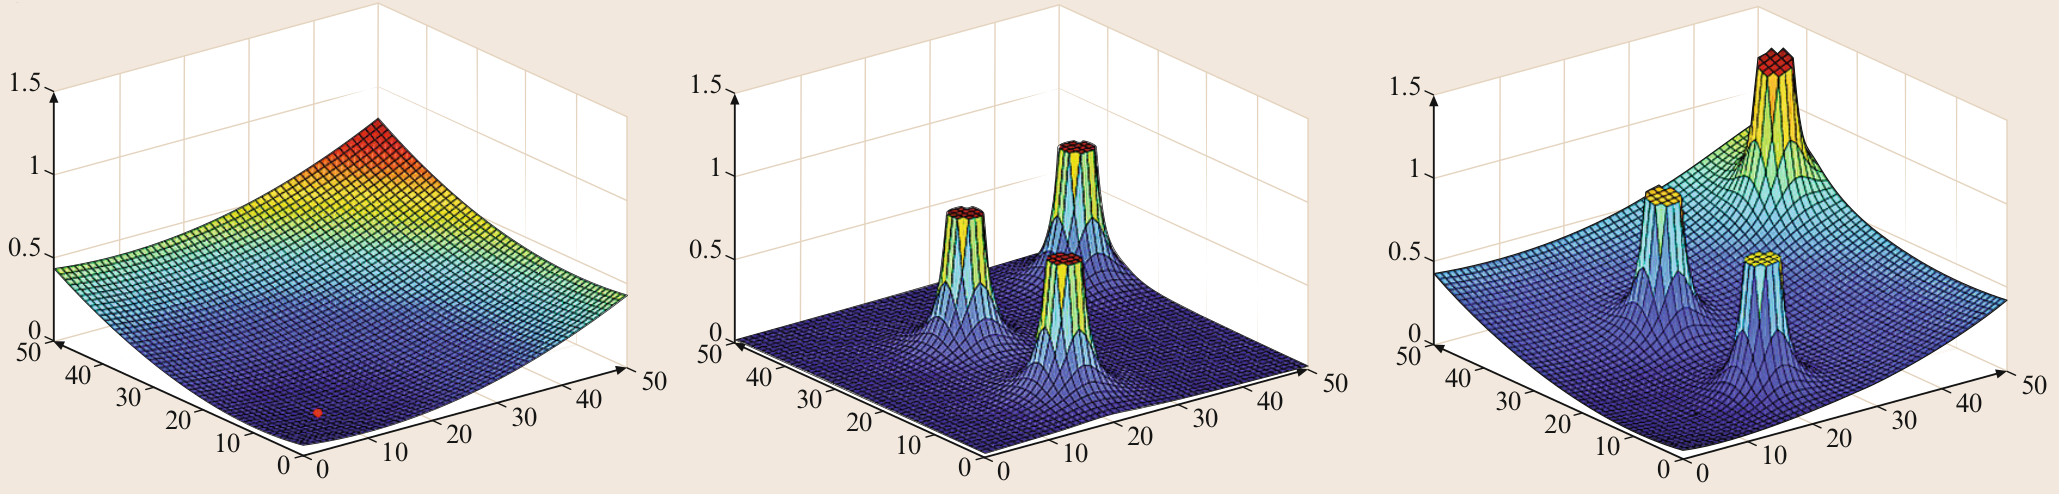
\includegraphics[width=\textwidth]{Figures/PotFieldsExample.png}
  \begin{itemize}
  \item \textbf{Campos repulsivos:} Por cada obstáculo se diseña una función $U_{rej_i}(q)$ con un máximo local en la posición $q_{o_i}$ del obstáculo.
  \item \textbf{Campo atractivo:} Se diseña una función $U_{att}(q)$ con un mínimo global en el punto meta $q_g$.
  \item La función potencial total $U(q)$ se calcula como
    \[ U(q) = U_{att}(q) + \frac{1}{N}\sum_{i=1}^N U_{rej_i}(q)\]
  \end{itemize}
\end{frame}

\begin{frame}\frametitle{Fuerzas atractiva y repulsivas}
  Puesto que el gradiente es un operador lineal, se pueden diseñar directamente las fuerzas atractiva $F_{att}(q) = \nabla U_{att}(q)$ y repulsivas $F_{rej_i}(q) = \nabla U_{rej_i}(q)$, de modo que la fuerza total será:
  \[ \nabla U(q) = F(q) = F_{att}(q) + \frac{1}{N}\sum_{i=1}^N F_{rej_i}(q)\]
  Una propuesta de estas fuerzas es:
  \begin{eqnarray*}
    \label{eq:attractive}
    F_{att} &=& \zeta \dfrac{\left(q - q_g\right) }{\Vert q - q_g \Vert},\qquad \zeta > 0\label{eq:PotFieldsAttraction}\\
    F_{rej} &=& \begin{cases}
                  \eta\left(\sqrt{\dfrac{1}{d} - \dfrac{1}{d_0}}\right)\dfrac{q_{o_i} - q}{d}
                  & \quad\textrm{si}\quad d < d_0\\
                  0 & \quad\textrm{en otro caso}
                \end{cases}
  \end{eqnarray*}
  donde
  \begin{itemize}
  \item $q=(x,y)$ es la posición del robot
  \item $q_g=(x_g, y_g)$ es el punto que se desea alcanzar
  \item $q_{o_i} = (x_{o_i}, y_{o_i})$ es la posición del $i$-ésimo obstáculo
  \item $d_0$ es una distancia de influencia. Más allá de $d_0$ los obstáculos no producen efecto alguno
  \item $\zeta$ y $\eta$, junto con $d_0$, son constantes de sintonización
  \end{itemize}
\end{frame}

\begin{frame}\frametitle{Evasión de obstáculos por campos potenciales}
  \begin{itemize}
  \item Aunque las ecuaciones anteriores suponen que se conoce la posición de cada obstáculo $q_{o_i}$, en realidad ésta aparece siempre en la diferencia $q_{o_i} - q$, es decir, solo se requiere su posición relativa al robot.
  \item Los campos potenciales se implementan utilizando el lidar, donde cada lectura se considera un obstáculo. 
  \end{itemize}
  \begin{figure}
    \centering
    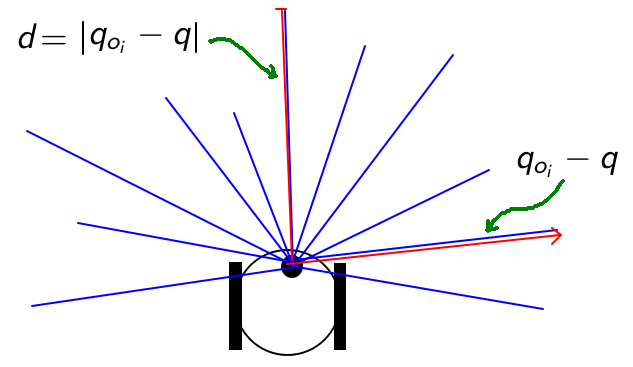
\includegraphics[width=0.4\textwidth]{Figures/PotFieldsLidar.png}
  \end{figure}
  Las lecturas del lídar generalmente son pares distancia-ángulo $(d_i,\theta_i)$ expresados con respecto al robot, por lo que, si se conoce la posición del robot $(x_r,y_r,\theta_r)$, la posición de cada obstáculo se puede calcular como:
  \begin{eqnarray*}
    x_{oi} &=& x_r + d_i\cos(\theta_i + \theta_r)\\
    y_{oi} &=& y_r + d_i\sin(\theta_i + \theta_r)\\
  \end{eqnarray*}
\end{frame}

\begin{frame}\frametitle{Evasión de obstáculos por campos potenciales}
  Finalmente, para que el robot alcance el punto de menor potencial, se puede emplear el descenso del gradiente:
  \[\]
  \begin{algorithm}[H]
  \DontPrintSemicolon
  \KwData{Posición inicial $q_s$, posición meta $q_g$, posiciones $q_{oi}$ de los obstáculos y tolerancia $tol$}
  \KwResult{Secuencia de puntos $\{q_0,q_1, q_2, \dots\}$ para evadir obstáculos y alcanzar el punto meta}
  \;
$q \leftarrow q_s$\;
\While{$\Vert\nabla U(q)\Vert > tol$}
{
  $q \leftarrow q - \epsilon F(q)$\;
  $[v,\omega] \leftarrow $ leyes de control con $q$ como posición deseada\;
}
  \caption{Descenso del gradiente para mover al robot a través de un campo potencial.}
  \label{alg:PotFields}
\end{algorithm}
\end{frame}

\begin{frame}\frametitle{Evasión de obstáculos por campos potenciales}
  Ejemplo de movimiento:
  \begin{figure}
    \centering
    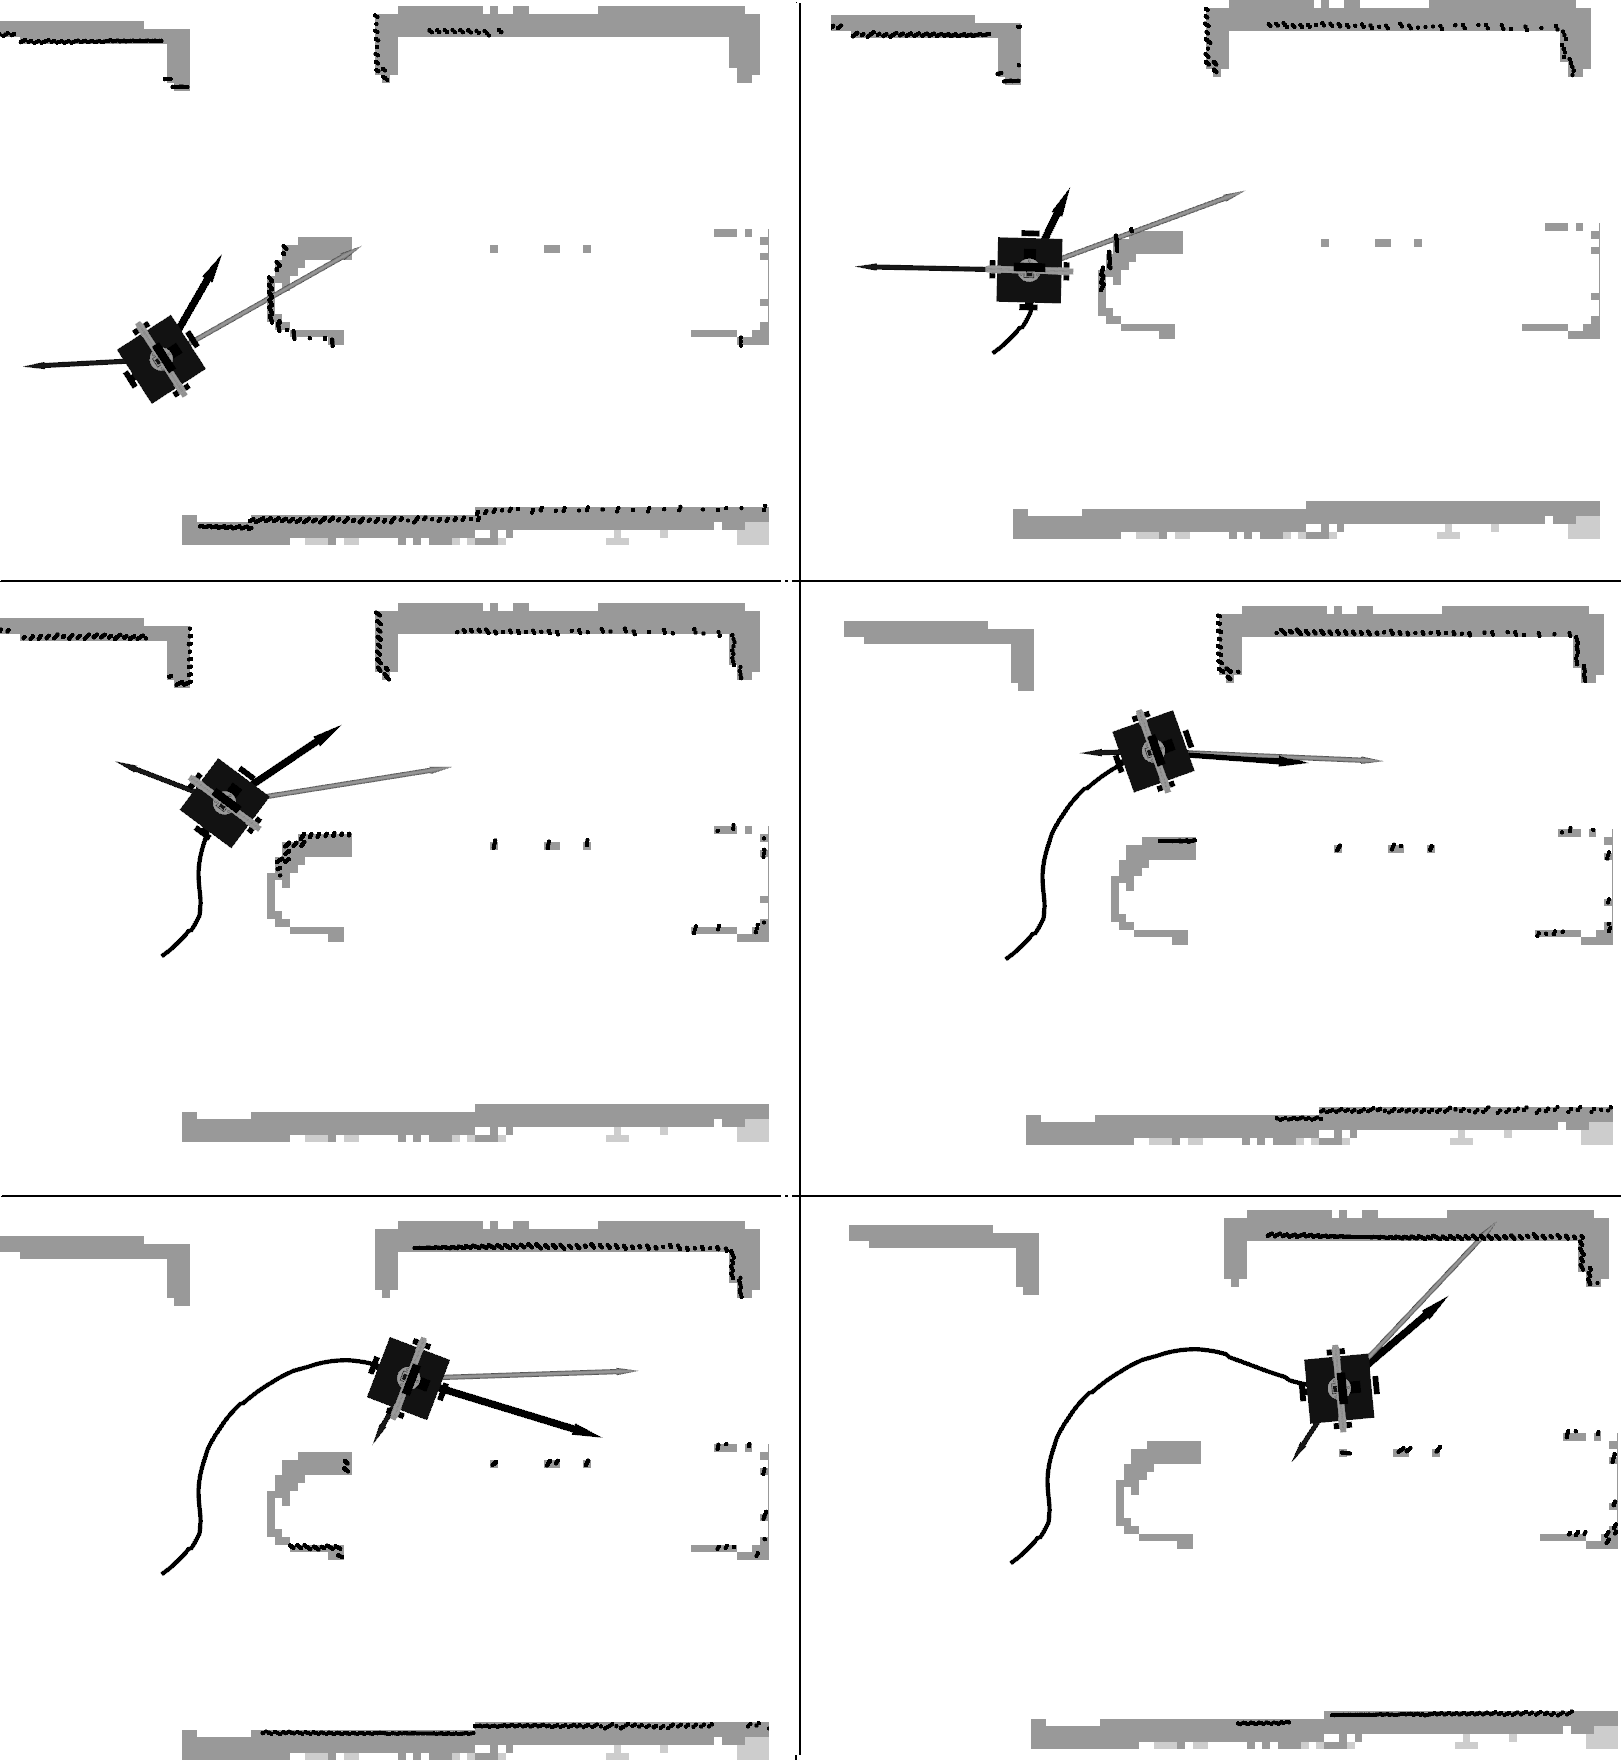
\includegraphics[height=0.85\textheight]{Figures/PotFieldsExecution.png}
  \end{figure}
\end{frame}

\begin{frame}[containsverbatim]\frametitle{Ejercicio 7 - Evasión de obstáculos}
  \begin{enumerate}
  \item Ejecute la simulación con el comando \texttt{roslaunch bring\_up obstacle\_avoidance.launch}
  \item Ejecute la evasión por campos potenciales mediante el comando\\ \texttt{rosrun exercises pot\_fields.py}
  \item Con la opción \textit{2D Nav Goal} del visualizador \textit{RViz}, selecccione un punto meta en el mapa.
  \item Observe el comportamiento.
  \item Detenga la ejecución de los campos potenciales. 
  \item Abra el archivo \texttt{catkin\_ws/src/exercises/scripts/pot\_fields.py} y modifique las constantes de atracción (línea 66), repulsión (línea 86) y distancia de influencia (línea 87)
  \item Ejecute nuevamente los campos potenciales y observe el cambio en el comportamiento.
  \end{enumerate}
\end{frame}

\begin{frame}\frametitle{Localización}
  El problema de la localización consiste en determinar la configuración $q$ del robot dada un mapa y un conjunto de lecturas de los sensores.
  \begin{itemize}
  \item La localización se podría lograr simplemente integrando los comandos de velocidad del robot.
  \item Si se conoce perfectamente la configuración inicial y el robot ejecuta perfectamente los comandos de movimiento, entonces la simple integración de la velocidad de los motores sería suficiente.
  \item Esto por supuesto no es posible. Se tiene incertidumbre tanto en la estimación inicial de la posición como en la ejecución de cada movimiento.
  \item Es decir, el robot pierde información sobre su posición en cada movimiento. 
  \end{itemize}
\end{frame}

\begin{frame}\frametitle{Localización}
  Existen principalmente dos tipos:
\[\]
  \begin{columns}
    \begin{column}{0.5\textwidth}
      \textbf{Localización local: }
      \begin{itemize}
      \item Requiere una estimación inicial \textit{cercana} a la posición real del robot, de otro modo, no converge.
      \item Suele ser menos costosa computacionalmente.
      \item Un método común es el Filtro de Kalman Extendido.
      \end{itemize}
    \end{column}
    \begin{column}{0.5\textwidth}
      \textbf{Localización global:}
      \begin{itemize}
      \item La estimación inicial puede ser cualquiera.
      \item Suele ser computacionalmente costosa.
      \item Un método común son los Filtros de Partículas. 
      \end{itemize}
      \[\]
      \[\]
    \end{column}
  \end{columns}
\end{frame}

\begin{frame}\frametitle{Localización probabilística}
  \begin{itemize}
  \item En la localización probabilística, en lugar de llevar una sola hipótesis sobre la posición del robot, se mantiene una \textit{distribución de probabilidad} sobre todo el espacio de hipótesis.
  \item El enfoque probabilístico permite manejar las incertidumbres inherentes al movimiento y al sensado.
  \item El reto es obtener una distribución de densidad de probabilidad (PDF) sobre todas las posibles posiciones del robot.
  \item En general, los métodos probabilísticos de estimación se componen de dos pasos:
    \begin{enumerate}
    \item \textbf{Predicción:} Se modifica la PDF de la posición del robot con base en los comandos y el modelo de movimiento.
    \item \textbf{Actualización:} Se corrige la predicción mezclando la información de PDF predicha con información de los sensores. Se obtiene una PDF de la posición y se repite el proceso. 
    \end{enumerate}
  \end{itemize}
  
\end{frame}

\begin{frame}\frametitle{Filtros de Partículas}
  \begin{figure}
    \centering
    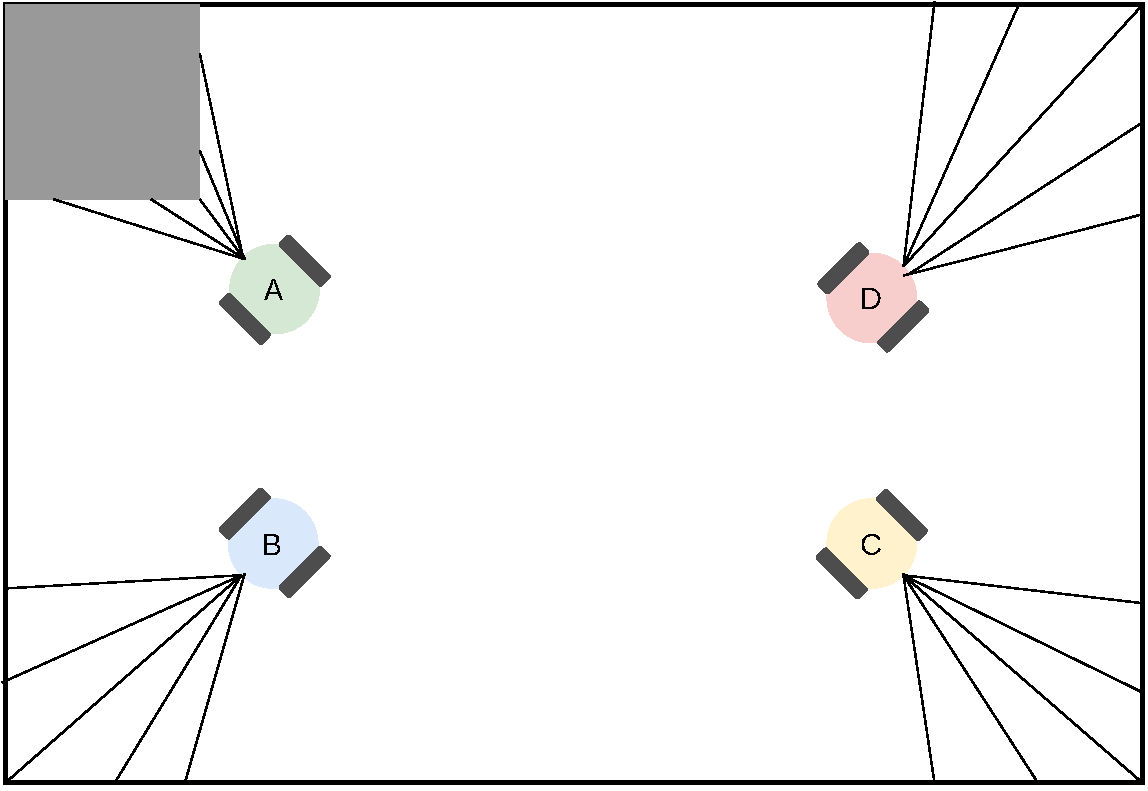
\includegraphics[width=0.6\textwidth]{Figures/ParticleFilter1.pdf}
  \end{figure}
\end{frame}

\begin{frame}[containsverbatim]\frametitle{Ejercicio 8 - Filtros de partículas}
  \begin{enumerate}
  \item Ejecute la simulación con el comando \texttt{roslaunch bring\_up localization.launch}
  \item Ejecute la localización por filtros de partículas mediante el comando \texttt{rosrun exercises particle\_filters}
  \item Con la GUI mueva el robot un poco hacia adelante. 
  \item Observe el comportamiento de las partículas conforme se mueve el robot. 
  \end{enumerate}
\end{frame}

\section{Visión}

\begin{frame}
  \Huge
  Visión
\end{frame}

\begin{frame}\frametitle{Las imágenes como funciones}
Una imagen (en escala de grises) es una función $I(x,y)$ donde $x,y$ son variables discretas en coordenadas de imagen y la función $I$ es intensidad luminosa. Las imágenes también pueden considerarse como arreglos bidimensionales de números entre un mínimo y un máximo (usualmente 0-255).
\begin{figure}
  \centering
  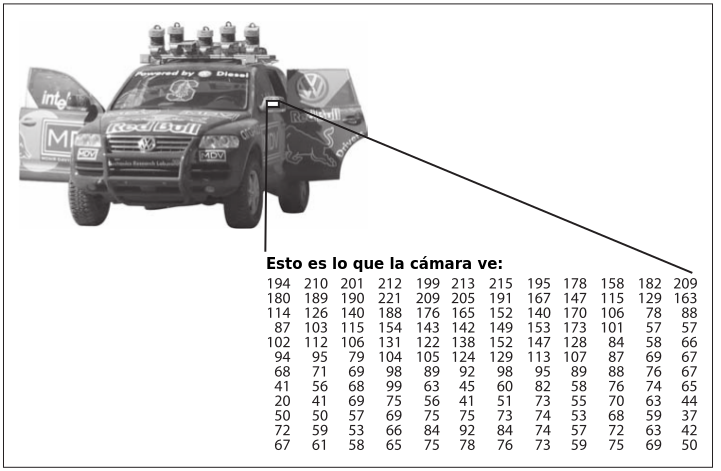
\includegraphics[width=0.45\textwidth]{Figures/representation_image.png}
\end{figure}
  Aunque formalmente una imagen es un mapeo $f:\mathbb{R}^2\rightarrow \mathbb{R}$, en la práctica, tanto $x,y$ como $I$ son varialbes discretas con valores entre un mínimo y un máximo.
\end{frame}

\begin{frame}\frametitle{Espacios de color}
  Las imágenes de color son funciones vectoriales $f:\mathbb{R}^2\rightarrow \mathbb{R}^3$ donde cada componente de la función se llama canal:
  \[I(x,y) = \left[\begin{tabular}{c}$r(x,y)$\\$g(x,y)$\\$b(x,y)$\end{tabular}\right]\]  
  Los espacios de color son diferentes formas de representar el color mediante la combinación de un conjunto de valores. 
  \begin{figure}
    \centering
    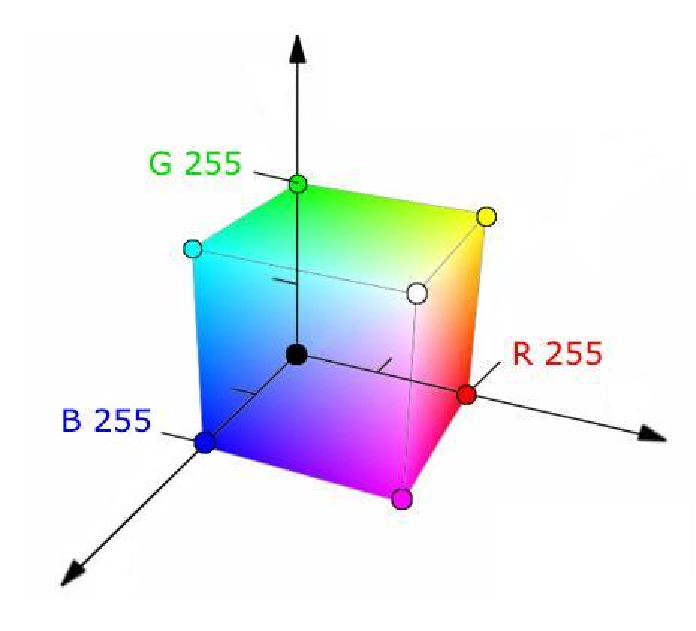
\includegraphics[width=0.33\textwidth]{Figures/RGB_model.pdf}
    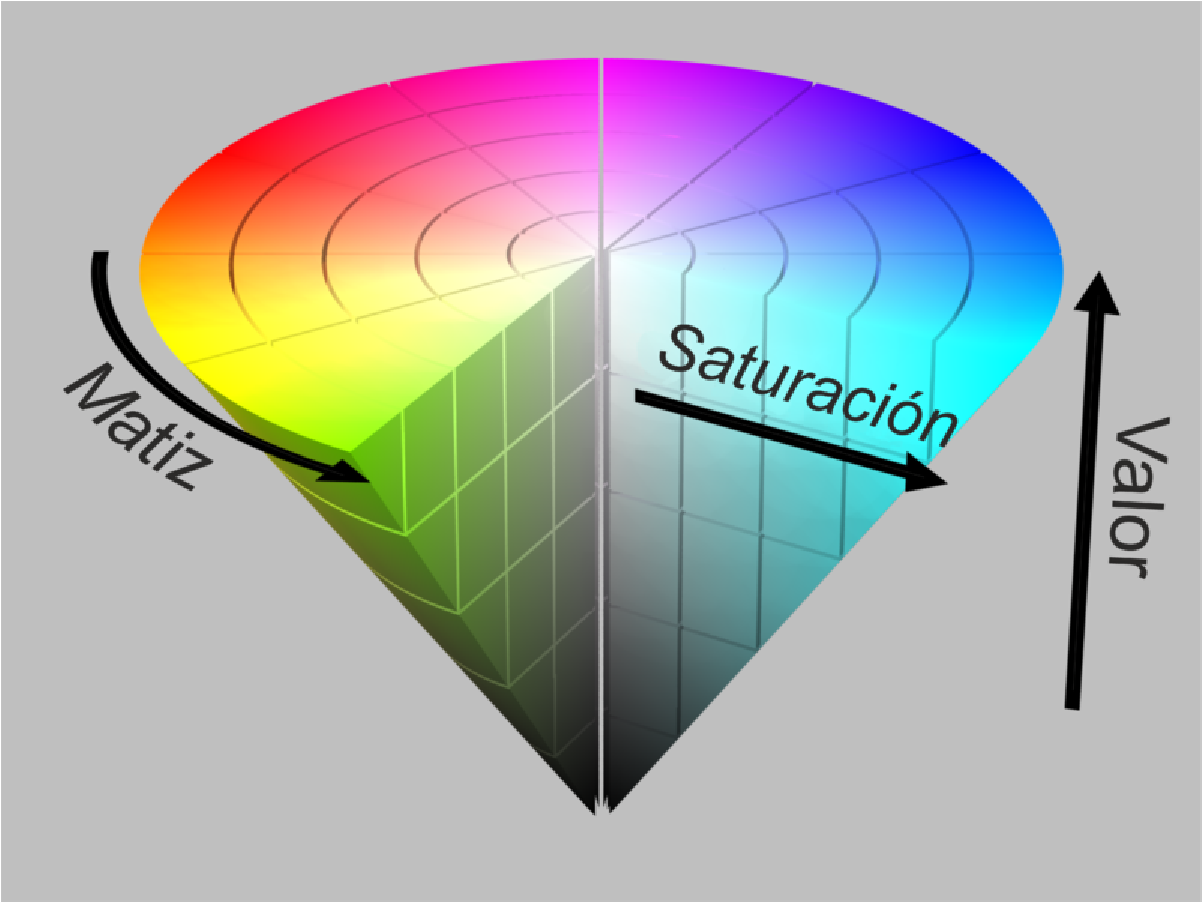
\includegraphics[width=0.33\textwidth]{Figures/hsv_space.pdf}
  \end{figure}
  En segmentación por color se recomienda más usar HSV, pues es más robusto ante cambios en la iluminación.
\end{frame}

\begin{frame}\frametitle{Nubes de puntos}
  Las nubes de puntos son conjuntos de vectores que representan puntos en el espacio. Estos vectores generalmente tienen información de posición $(x,y,z)$. También pueden contener información de color $(x,y,z,r,g,b)$.
  \begin{figure}
      \centering
      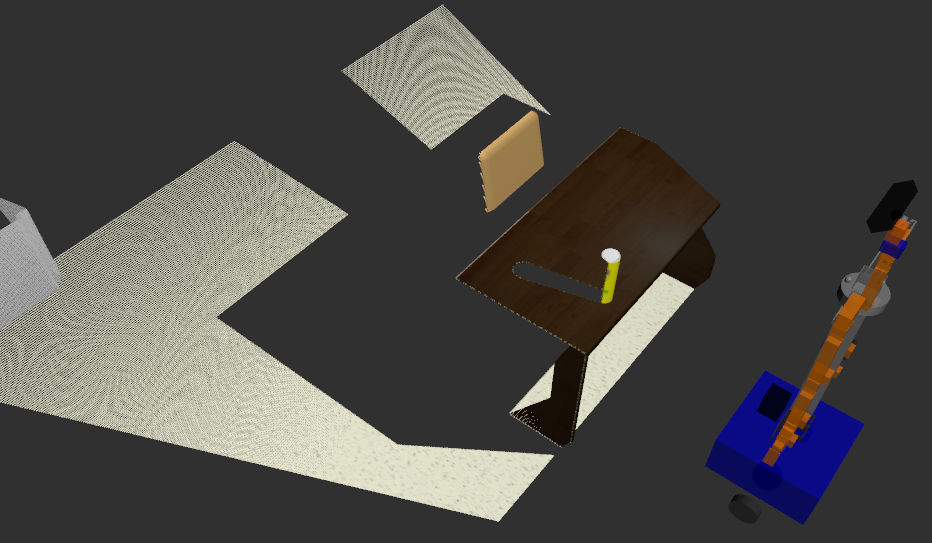
\includegraphics[width=0.5\textwidth]{Figures/CloudExample.png}
  \end{figure}
  Son útiles para determinar la posición en el espacio de los objetos reconocidos. 
\end{frame}

\begin{frame}\frametitle{OpenCV}
  \begin{itemize}
  \item OpenCV es un conjunto de bibliotecas que facilita la implementación de algoritmos de visión computacional.
  \item Se puede usar con diversos lenguajes: C++, Python, Java.
  \item En Python utiliza la biblioteca Numpy.
  \item Las imágenes se representan como matrices donde cada elemento puede ser un solo valor, o bien tres valores, dependiendo de si la imagen está en escala de grises o a color.
  \item La configuración más común es que cada pixel esté representado por tres bytes.
  \item Las nubes de puntos se representan también como matrices donde cada elemento es una terna de flotantes con la posición $(x,y,z)$.
  \end{itemize}
\end{frame}

\begin{frame}\frametitle{Segmentación por color}
  La segmentación de una imagen se refiere a obtener regiones significativas con ciertas características. En este caso, la característica es que estén en un cierto intervalo de color. Los pasos generales para esto son:
  \begin{enumerate}
  \item Transformación de la imagen del espacio BGR al HSV (función \texttt{cvtColor})
  \item Obtención de aquellos pixeles que están en un rango de color (función \texttt{inRange})
  \item Eliminación de \textit{outliers}, generalmente con operadores morfológicos (funciones \texttt{erode} y \texttt{dilate})
  \item Obtención del centroide de la región (funciones \texttt{findNonZero} y \texttt{mean})
  \item Si se dispone de una nube de puntos, se puede obtener la posición $(x,y,z)$ del centroide de la región segementada. 
  \end{enumerate}
\end{frame}

\begin{frame}[containsverbatim]\frametitle{Ejercicio 9 - Segmentación por color}
  Ejecute la simulación con el comando:
  \begin{lstlisting}
    roslaunch bring_up color_segmentation.launch
  \end{lstlisting}
  Y en otra terminal ejecute la segmentación por color:
  \begin{lstlisting}
    rosrun exercises color_segmentation.py
  \end{lstlisting}
  Utilizando la GUI, baje la cabeza del robot hasta que los objetos del escritorio estén en el campo visual:
  \begin{figure}
    \centering
    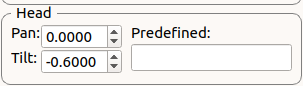
\includegraphics[width=0.35\textwidth]{Figures/Exercise5Gui1.png}
  \end{figure}
  En la pestaña \textit{Simple Tasks}, teclee las palabras ``pringles'' o ``drink'' en el campo \textit{Find Object}. Observe el resultado en el visualizador RViz. 
\end{frame}


\section{Manipulación}

\begin{frame}
  \Huge
  Manipulación
\end{frame}

\begin{frame}\frametitle{Posición y Orientación}
  Un cuerpo rígido en el espacio puede tener una posición $(x,y,z)$ y una orientación. La orientación se puede representar de varias formas:
  \begin{itemize}
  \item Mediante ángulos de Euler: roll, pich y yaw $RPY = (\psi, \theta, \phi)$
  \item Mediante cuaterniones
  \item Mediante una matriz de rotación $R \in SO(3)$
  \end{itemize}
  Los ángulos $RPY$ son rotaciones intrínsecas sobre los ejes $X$, $Y$, y $Z$ respectivamente. Se llaman intrínsecas porque son rotaciones que ocurren sobre un sistema de referencia \textit{atado} a un cuerpo rígido.\\
  Cualquier orientación se puede obtener mediante la composición de tres rotaciones básicas:
  \[R = R_{z,\phi}R_{y,\theta}R_{x,\psi}\]
  Es decir, primero una rotación de $\phi$ radianes sobre el eje $Z$, seguida de una rotación de $\theta$ radianes sobre el eje $Y$ del sistema resultante y una rotación de $\psi$ radianes sobre el eje $X$ del sistema rotado. 
\end{frame}

\begin{frame}\frametitle{Transformaciones Homogéneas}
  Una Transformación Homogénea es una matriz de la forma
  \[T = \left[\begin{tabular}{cccc}
      & & & $d_x$\\
      & $R\in SO(3)$ & & $d_y$\\
      & & & $d_z$\\
      0 & 0& 0 & 1
    \end{tabular}\right]\]
  Puede servir para
  \begin{itemize}
  \item Representar la posición y orientación de un cuerpo rígido
  \item Representar una transformación de coordenadas $T_{ab}$ de un sistema de referencia $b$ a un sistema $a$
  \end{itemize}
  Propiedades:
  \begin{itemize}
  \item Asociatividad: $(T_1 T_2) T_3 = T_1 (T_2 T_3)$
  \item Inversa:
    \[T = \left[\begin{tabular}{cc}
       $R^T$ & $-R^T d$\\
       0 & 1
      \end{tabular}\right]\]
  \item Cancelación de índices: $T_{ab} = T_{ac}T_{cb}$
  \end{itemize}
\end{frame}

\begin{frame}\frametitle{El árbol cinemático}
  Es útil tener una descripción de la forma en que están conectadas las diferentes articulaciones del robot. Se considera que sobre cada articulación hay un sistema de referencia (\textit{frame}) que está trasladado y rotado con respecto al sistema anterior.
  \begin{multicols}{3}
    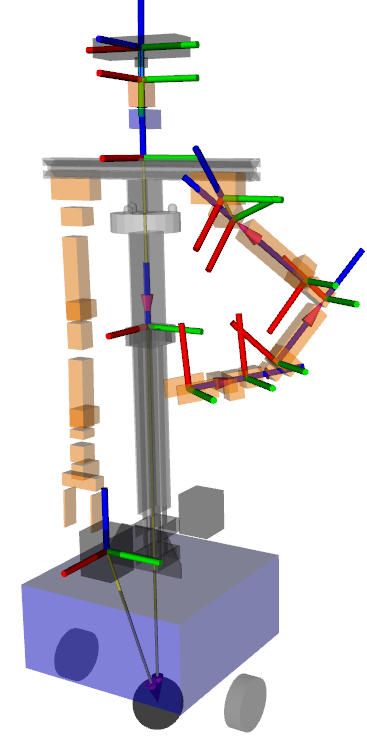
\includegraphics[width=0.26\textwidth]{Figures/KinematicTree.png}\\
    \footnotesize
    El sistema \textit{absoluto} se suele llamar \texttt{map}\\
    El sistema base del robot se suele llamar \textit{base\_link}\\
    Las transformaciones de \texttt{map} a \texttt{base\_link} las determina el sistema de localización\\
    El resto de las transformaciones se determinan con la posición de cada articulación\\
    El árbol cinemático se traduce en una cadena de mulplicaciones de Transformaciones Homogéneas. 
    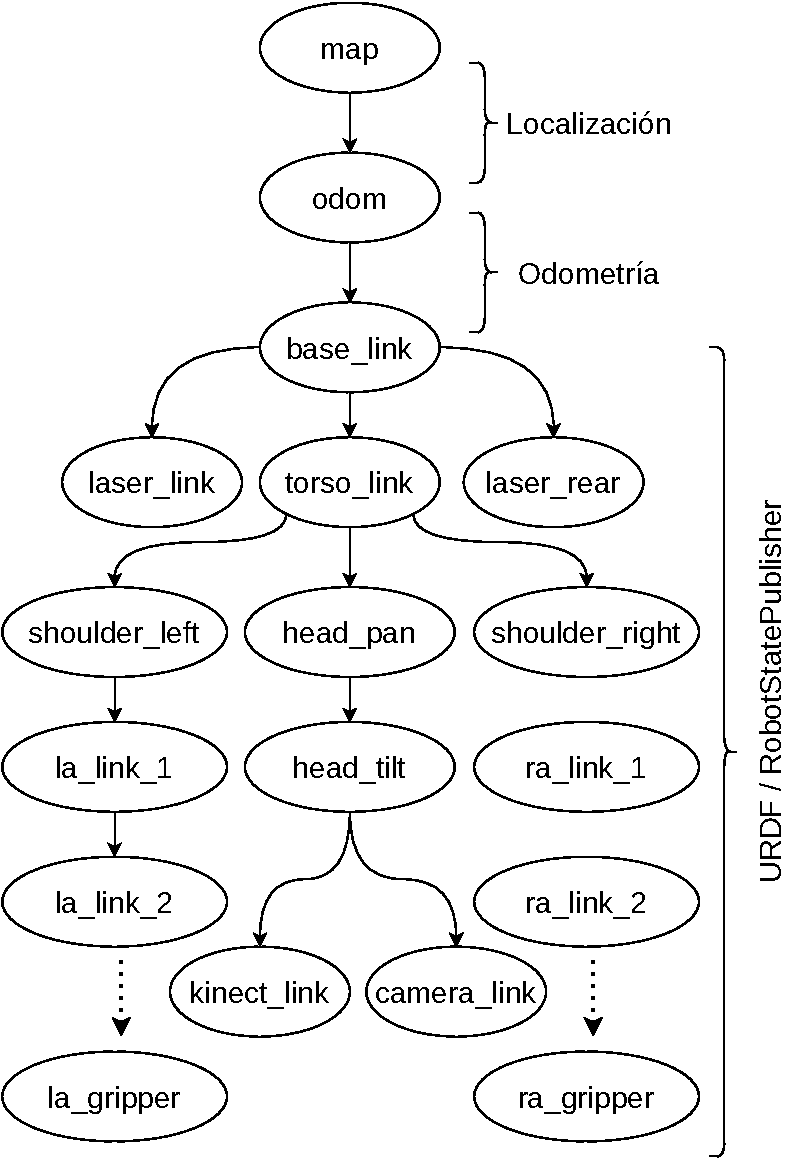
\includegraphics[width=0.35\textwidth]{Figures/TfTree.pdf}
  \end{multicols}
\end{frame}

\begin{frame}[containsverbatim]\frametitle{El formato URDF}
  El formato URDF permite describir el arbol cinemático del robot mediante etiquetas XML:
  \footnotesize
  \lstinputlisting[language=XML]{Codes/URDFExample.xml}
  \normalsize
  Cada etiqueta \texttt{<joint>} representará una Transformación Homogénea. 
\end{frame}

\begin{frame}[containsverbatim]\frametitle{El formato Xacro}
  El formato Xacro es un lenguaje de \textit{macros} que permite obtener archivos XML más cortos. Es últil para especificar parámetros físicos en el URDF como inercias y volúmenes:
  \footnotesize
  \lstinputlisting[language=XML]{Codes/XacroExample.xml}
\end{frame}

\begin{frame}[containsverbatim]\frametitle{Ejercicio 10 - Formato Xacro}
  Abra el archivo \texttt{catkin\_ws/src/hardware/justina\_description/urdf/justina.xacro} y modifique la línea 17 de acuerdo con lo siguiente:
  \lstinputlisting[language=XML,firstnumber=16]{Codes/JustinaXacro.xml}
  Ejecute la simulación:
  \begin{lstlisting}
    roslaunch bring_up path_planning.launch
  \end{lstlisting}
  Detenga la simulación. Regrese las variables a sus valores originales.
\end{frame}

\begin{frame}\frametitle{La cinemática directa}
  La cinemática directa consiste en determinar la posición y orientación del efector final del manipulador a partir de la posición de cada articulación.  Esta se puede calcular con la ecuación:
  \[P_1 = T_{12}T_{23}T_{34}T_{45}T_{56}T_{67}T_{7g}P_g\]
  donde $P_g = [0,0,0,1]^T$ es la posición del gripper con respecto al sistema del gripper, $P_1$ es la posición del gripper con respecto al sistema base y $T_{ab}$ es la transformación homogénea que define la rotación y traslación producida por cada articulación. Las matrices $T_{ab}$
  tienen la forma:
  \[T_{ab} = \left[\begin{tabular}{cccc}
      & & & $dx_{ab}$\\
      & $R_{ab}\in SO(3)$ & & $dy_{ab}$\\
      & & & $dz_{ab}$\\
      0 & 0& 0 & 1
    \end{tabular}\right]\]
  Donde $R_{ab}$ representa la rotación del sistema $b$ respecto al sistema $a$ y $(dx_{ab}, dy_{ab}, dz_{ab})$ es la traslación del sistema $b$ respecto al sistema $a$.\\
  La rotación $R_{ab}$ está definida en el URDF por el atributo ``rpy'' de la sub etiqueta \texttt{origin} de la etiqueta \texttt{joint} y por la posición de la articulación. La traslación $(dx_{ab}, dy_{ab}, dz_{ab})$ está definida por el atributo ``xyz''. 
\end{frame}

\begin{frame}[containsverbatim]\frametitle{Ejercicio 11 - Cinemática directa}
  \begin{itemize}
  \item Ejecute la simulación con el comando \texttt{roslaunch bring\_up inverse\_kinematics.launch}
  \item Ejecute el cálculo de la cinemática: \texttt{rosrun exercises inverse\_kinematics.py}
  \end{itemize}
  En la GUI, mueva las articulaciones con los controles del bloque \textit{Articular} y observe los cambios en la etiqueta \textit{Current} del bloque \textit{Cartesian}
  \begin{figure}
    \centering
    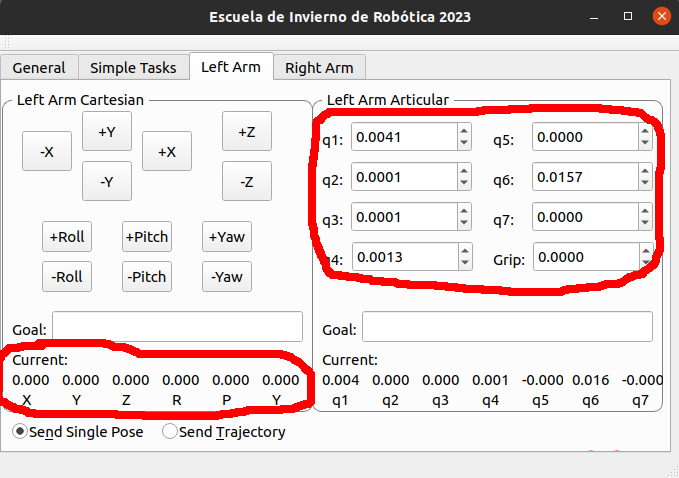
\includegraphics[width=0.6\textwidth]{Figures/ForwardKinematics.png}
  \end{figure}
\end{frame}


\begin{frame}\frametitle{La cinemática inversa}
  La cinemática inversa consiste en determinar las posiciones que debe tener cada articulación para que el efector final tenga la posición y orientación deseadas.
  \begin{itemize}
  \item Mientras la cinemática directa siempre tiene solución, la cinemática inversa, no.
  \item Se puede resolver por métodos geométricos para obtener una solución cerrada, aunque el análisis puede ser muy complicado.
  \item Una solución más general se puede obtener mediante un método numérico. 
  \end{itemize}
  Suponiendo que se tiene una configuración deseada $p_d \in \mathbb{R}^6$ ($xyz-RPY$), se desea encontrar el conjunto de posiciones articulares $q\in\mathbb{R}^7$ que satisfagan la ecuación
  \[FK(q) - p_d = 0\]
  donde la función $FK$ representa la cinemática directa. 
\end{frame}

\begin{frame}\frametitle{El método Newton-Raphson}
  El método numérico de Newton-Raphson sirve para encontrar raíces, es decir, para resolver ecuaciones de la forma
  \[f(x) = 0\]
  El algoritmo es el siguiente:
  \[\]
  \begin{multicols}{2}
  \begin{algorithm}[H]
    \DontPrintSemicolon
    $x_i \leftarrow x_0$\;
    \While{$|f(x)| > \epsilon$}
    {
       $x_{i+1} \leftarrow x_i - \frac{f(x_i)}{f'(x_i)}$
    }
  \end{algorithm}
  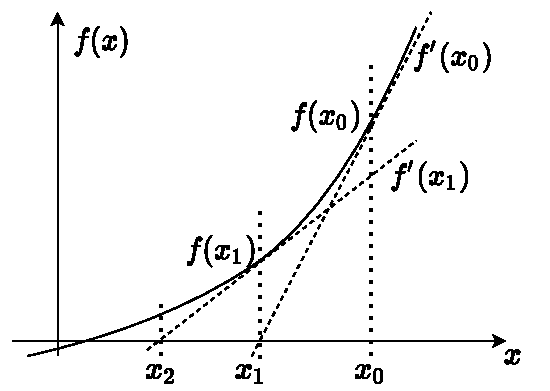
\includegraphics[width=0.4\textwidth]{Figures/NewtonRaphson.pdf}
  \end{multicols}
\end{frame}

\begin{frame}\frametitle{El Jacobiano}
  El Jacobiano es una matriz que relaciona la velocidad articular $\dot{q}$ con la velocidad en el espacio cartesiano $[v\;\omega]^T$ (velocidad lineal y angular):
  \[\dot{p} = \left[\begin{tabular}{c}$v$\\$\omega$\end{tabular}\right] = J \dot{q}
  \qquad\qquad p = [x,y,z,roll, pitch, yaw] \in \mathbb{R}^6, \quad J\in \mathbb{R}^{6\times 7},\quad q\in \mathbb{R}^7\]
  \[J = \left[ \begin{tabular}{ccc}
      $\frac{\partial p_1}{\partial q_1}$ & $\cdots$ & $\frac{\partial p_1}{\partial q_7}$\\
      $\vdots$ & $\ddots$ & $\vdots$ \\
      $\frac{\partial p_6}{\partial q_1}$ & $\cdots$ & $\frac{\partial p_6}{\partial q_7}$\\
    \end{tabular} \right]\]
  \begin{itemize}
  \item La matriz $J$ se puede obtener analíticamente, sin embargo, dado el número de grados de libertad, resulta muy complicado
  \item Se puede obtener aproximando las derivadas parciales con diferencias finitas:
  \end{itemize}
  \[J = \left[\frac{FK(q^1_{+}) -  FK(q^1_{-})}{2\Delta q} \qquad \cdots \qquad \frac{FK(q^7_{+}) -  FK(q^7_{-})}{2\Delta q}\right]\]
  \begin{eqnarray*}
    q^i_+ &=& [q_1\quad \dots \quad q_i + \Delta q \quad \dots \quad q_7]\\
    q^i_- &=& [q_1\quad \dots \quad q_i - \Delta q \quad \dots \quad q_7]
  \end{eqnarray*}
  con $\Delta q$, un valor lo suficientemente pequeño para una buena aproximación de la derivada. 
\end{frame}

\begin{frame}\frametitle{Cinemática Inversa por Newton-Raphson}
  Aplicando Newton-Raphson para resolver la ecuación:
  \[FK(q) - p_d = 0\]
  Se tiene:
  \begin{algorithm}[H]
    \DontPrintSemicolon
    $q_i \leftarrow q_0$ //Una estimación inicial que puede ser la posición articular actual\;
    $p \leftarrow FK(q_i)$ //La posición cartesiana que tendría el gripper con la estimación inicial\;
    \While{$|p - p_d| > \epsilon$}
    {
      $J \leftarrow Jacobiano(q)$     \;
      $q_{i+1} \leftarrow q_i - J^\dagger (p - p_d)$\;
      $p \leftarrow FK(q_i)$ 
    }
  \end{algorithm}
  Puesto que el Jacobiano $J$ no es una matriz cuadrada, no tiene inversa, por lo que se utiliza la matriz pseudoinversa $J^\dagger$. 
  \begin{itemize}
  \item Es importante que las variables angulares siempre estén en el intervalo $(-\pi, \pi]$:
    \begin{itemize}
    \item Las posiciones articulares
    \item Los ángulos roll, pitch, yaw
    \item Las componentes angulares del error $p - p_d$
    \end{itemize}
  \end{itemize}
\end{frame}

\begin{frame}[containsverbatim]\frametitle{Ejercicio 12 - Cinemática inversa}
  \begin{itemize}
  \item Ejecute la simulación con el comando \texttt{roslaunch bring\_up inverse\_kinematics.launch}
  \item Ejecute el cálculo de la cinemática inversa: \texttt{rosrun exercises inverse\_kinematics.py}
  \end{itemize}
  En la GUI, en el campo \textit{goal} del bloque \textit{articular}, escriba ``prepare'' (en cualquiera de los dos brazos):
  \begin{figure}
    \centering
    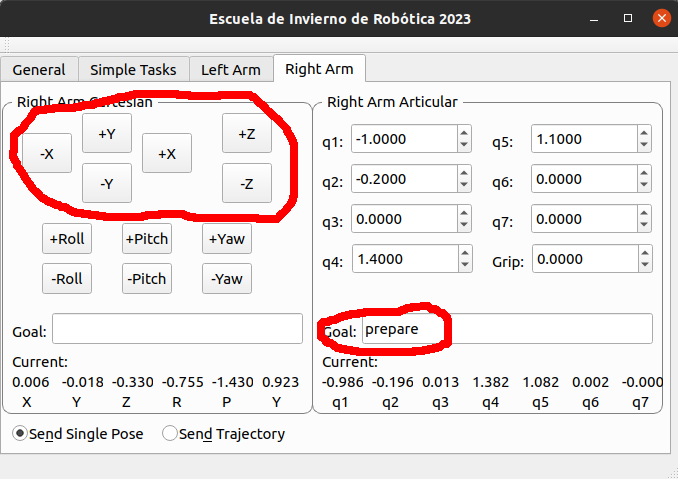
\includegraphics[width=0.6\textwidth]{Figures/InverseKinematics.png}
  \end{figure}
  Utilice los controles del bloque \textit{cartesian} para mover el manipulador.
\end{frame}

\begin{frame}\frametitle{El control PID}
  El control Proporcional-Integral-Derivativo es un tipo de control lineal en lazo cerrado que calcula la acción de control mediante una combinación lineal del error, la integral del error y la derivada del error.
  \begin{itemize}
  \item Para el manipulador, el ángulo deseado $q_d$ está dado por el resultado de la cinemática inversa. 
  \item La posición angular $q$ se obtiene de los motores o del simulador.
  \item La salida del controlador es el torque $\tau$ que se envía a los motores.
  \end{itemize}
  En la versión continua:
  \[\tau(t) = K_p e(t) + K_I \int e(t)dt + K_d \dot{e}(t)\]
  con $e = q_d - q$
  En la versión discreta:
  \[\tau_i = K_p e_i + K_I\sum_{j=0}^i e_j + K_d\frac{e_i - e_{i-1}}{\Delta t}\]
  con $\Delta t$, el periodo de muestreo. 
\end{frame}

\begin{frame}\frametitle{El control PID}
  Aunque la interacción de las tres señales (error, integral del error y derivada del error) es compleja y depende mucho del sistema, de manera intuitiva se pueden indicar las siguientes funciones de cada componente:
  \begin{itemize}
  \item \textbf{Proporcional:} Aumenta o disminuye el tiempo de asentamiento.
  \item \textbf{Integral:} Reduce el error en estado estable, aunque puede producir inestabiliddad.
  \item \textbf{Derivativa:} Funciona como amortiguamiento y ayuda a disminuir el sobrepaso. 
  \end{itemize}
\end{frame}

\begin{frame}\frametitle{Los \textit{stacks} ros\_control y ros\_controllers}
  Son un conjunto de paquetes que implementan controladores PID y varias interfaces de hardware.
  \begin{itemize}
  \item El stack \texttt{ros\_control} implementa varias interfaces de hardware. En este curso, la interfaz usada es la que interactúa con la simulación de Gazebo. De este stack, el paquete \texttt{controller\_manager} es importante porque utiliza un archivo \textit{yaml} para lanzar otros nodos que implementan controladores PID. 
  \item El stack \texttt{ros\_controllers} implementa varios algoritmos de control para diferentes tipos de actuadores. 
  \end{itemize}
\end{frame}

\begin{frame}[containsverbatim]\frametitle{Ejercicio 13 - Control PID}
  Ejecute el comando:
  \begin{lstlisting}
    roslaunch bring_up inverse_kinematics.launch
  \end{lstlisting}
  \begin{itemize}
  \item Utilizando la GUI, mueva las articulaciones de los manipuladores a alguna posición diferente de cero y observe el comportamiento.
  \item Abra el archivo \texttt{src/config\_files/ros\_control/justina\_controllers.yaml} y modifique las ganancias de los diferentes controladores. Detenga la simulación y ejecútela de nuevo. Compare el comportamiento.
  \end{itemize}
\end{frame}

\section{Síntesis de Voz}

\begin{frame}
  \Huge
  Síntesis de Voz
\end{frame}

\begin{frame}\frametitle{Síntesis de voz con SoundPlay}
  \begin{itemize}
  \item Es un paquete que permite reproducir archivos \texttt{.wav} o \texttt{.ogg}, sonidos predeterminados y síntesis de voz.
  \item La síntesis de voz se hace utilizando Festival (\url{http://www.cstr.ed.ac.uk/projects/festival/}).
  \item Para sintetizar voz, basta con correr el nodo \texttt{soundplay\_node} y publicar un mensaje de tipo \texttt{sound\_play/SoundRequest} con lo siguiente:
    \begin{itemize}
    \item msg\_speech.sound   = -3                 
    \item msg\_speech.command = 1                  
    \item msg\_speech.volume  = 1.0                
    \item msg\_speech.arg2    = ``voz a utilizar''
    \item msg\_speech.arg = ``texto a sintetizar''
    \end{itemize}
  \end{itemize}
\end{frame}

\begin{frame}[containsverbatim]\frametitle{Ejercicio 14 - Síntesis de voz}
  Ejecute el comando:
  \begin{lstlisting}
    roslaunch bring_up speech_synthesis.launch
  \end{lstlisting}
  En otra terminal, ejecute el comando:
  \begin{lstlisting}
    rosrun exercises speech_synthesis.py "my first synthetized voice"
  \end{lstlisting}
  Para instalar más voces:
  \begin{itemize}
  \item Ejecute el comando \texttt{sudo apt-get install festvox-<voz deseada>}
  \item Para ver qué voces se tienen instaladas: \texttt{ls /usr/share/festival/voices/english/}
  \end{itemize}
\end{frame}

\begin{frame}[containsverbatim]\frametitle{Ejercicio 14 - Síntesis de voz}
  Modifique el archivo \texttt{catkin\_ws/src/exercises/scripts/speech\_synthesis.py} y cambie la voz a utilizar en el mensaje SoundRequest.
  \lstinputlisting[language=Python,firstnumber=17]{Codes/SpeechSynthesis.py}
  El nombre de la voz se compone de \texttt{voice\_} más el nombre que aparece en la carpeta \texttt{/usr/share/festival/voices/english/}. 
\end{frame}

\section{Reconocimiento de voz}

\begin{frame}
  \Huge
  Reconocimiento de voz
\end{frame}

\begin{frame}\frametitle{Reconocimiento de voz con Pocketsphinx}
  Pocketsphinx es un \textit{toolkit} open source desarrollado por la Universidad de Carnegie Mellon (\url{https://cmusphinx.github.io/}).
  \begin{itemize}
  \item Aunque el toolbox original no está hecho específicamente para ROS, ya existen varios repositorios con nodos ya implementados que integran ROS y Pocketsphinx:
    \begin{itemize}
    \item \url{https://github.com/mikeferguson/pocketsphinx}
    \item \url{https://github.com/Pankaj-Baranwal/pocketsphinx}
    \end{itemize}
  \item El usuario debe estar agregado al grupo \textit{audio} para el correcto funcionamiento: \texttt{sudo usermod -a -G audio <user\_name>}
  \end{itemize}
  \begin{itemize}
  \item Se puede hacer reconocimiento usando una lista de palabras, un modelo de lenguaje o una gramática.
  \item Se utilizarán gramáticas y sus correspondientes diccionarios.
  \item Para construir diccionarios, visitar \url{https://cmusphinx.github.io/wiki/tutorialdict/}
  \item Para construir gramáticas, visitar \url{https://www.w3.org/TR/2000/NOTE-jsgf-20000605/}
  \end{itemize}
\end{frame}

\begin{frame}\frametitle{Ejercicio 10}
  \begin{enumerate}
  \item Verifique el volumne del micrófono
  \item Inspeccione el archivo \texttt{catkin\_ws/src/pocketsphinx/vocab/gpsr.gram} para ver las frases que se pueden reconocer de acuerdo con la gramática.
  \item Ejecute el comando \texttt{roslaunch bring\_up speech\_recognition.launch}
  \item En otra terminal, ejecute el comanto \texttt{rostopic echo /recognized}
  \item Pruebe el reconocimiento de voz con alguna de las siguientes frases:
    \begin{enumerate}
    \item \texttt{Robot, take the pringles to the table}
    \item \texttt{Robot, take the drink to the table}
    \item \texttt{Robot, take the pringles to the kitchen}
    \item \texttt{Robot, take the drink to the kitchen}
    \end{enumerate}
  \end{enumerate}
\end{frame}

\section{Planeación de acciones}

\begin{frame}
  \Huge
  Planeación de acciones
\end{frame}

\begin{frame}\frametitle{Máquinas de estados finitas}
  Las FSM son modelos que permiten representar procesos discretos donde el sistema puede estar en un estado bien definido y existen un conjunto de reglas para definir el estado siguiente en función del estado actual y las entradas. Opcionalmente, se pueden definir salidas para cada estado. \\
  Formalmente, una FSM está definida por:
  \begin{itemize}
  \item $S$ : Conjunto finito no vacío de estados
  \item $\Sigma$ : Conjunto finito no vacío de entradas
  \item $s_0 \in S$ : Estado inicial
  \item $\delta : S\times\Sigma\rightarrow S$ : Función de transición de estados
  \item $F$ : Conjunto de estados finales (puede ser un conjunto vacío)
  \end{itemize}
\end{frame}

\begin{frame}\frametitle{Carta ASM}
  Una forma de representar los estados y transiciones de una FSM es mediante una carta ASM. Ejemplo:
  \begin{figure}
    \centering
    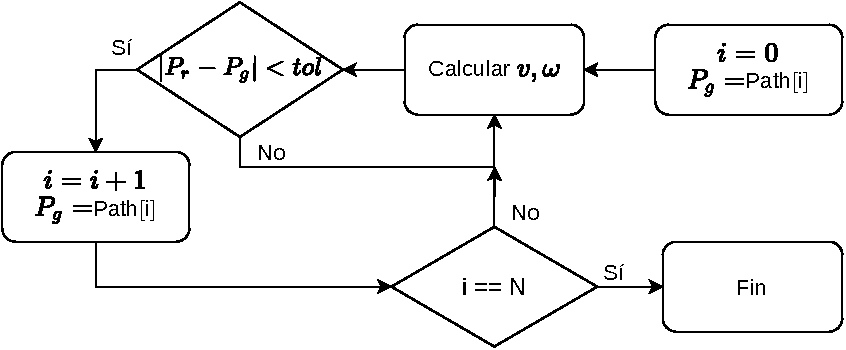
\includegraphics[width=0.6\textwidth]{Figures/PathFollowing.pdf}
  \end{figure}
  Las máquinas de estados se pueden utiizar para ejecutar tareas ``sencillas'' en un robot de servicio doméstico. 
\end{frame}

\begin{frame}\frametitle{FSM para manipular objetos}
  En cada estado podemos enviar comandos de movimiento y utilizar resultados de percepción para definir el siguiente estado:
  \begin{figure}
    \centering
    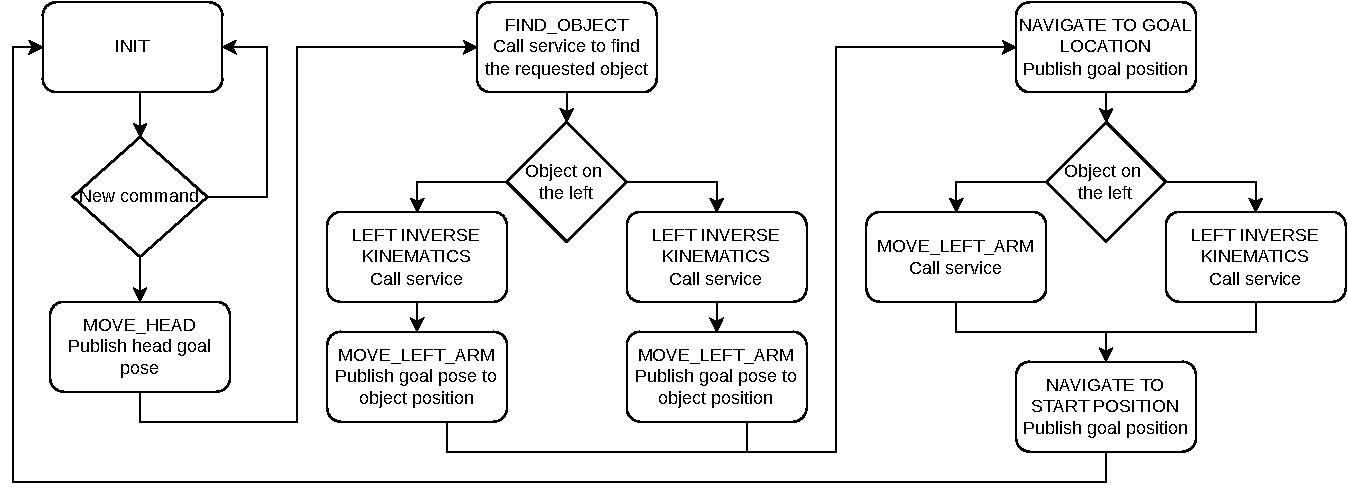
\includegraphics[width=\textwidth]{Figures/FSM.pdf}
  \end{figure}
\end{frame}

\begin{frame}[containsverbatim]\frametitle{Ejercicio Final}
  Abra el archivo \texttt{catkin\_ws/src/exercises/scripts/simple\_service\_robot.py} e inspeccione los diversos estados. Ejecute el comando:
  \begin{lstlisting}
    roslaunch bring_up final_exercise.launch
  \end{lstlisting}
  Y en otra terminal, corra la plneación para un robot de servicio simple:
  \begin{lstlisting}
    rosrun exercises simple_service_robot.py
  \end{lstlisting}
\end{frame}

\bibliographystyle{abbrv}
\bibliography{References}
\begin{frame}
  \Huge{Gracias}
  \[\]
  \Large{Contacto}
  \[\]
  \large
  Dr. Marco Negrete\\
  Profesor Asociado C\\
  Departamento de Procesamiento de Señales\\
  Facultad de Ingeniería, UNAM.
\[\]
mnegretev.info\\
marco.negrete@ingenieria.unam.edu\\
\end{frame}
\end{document}
